\documentclass{mimosis}

\usepackage{metalogo}

%%%%%%%%%%%%%%%%%%%%%%%%%%%%%%%%%%%%%%%%%%%%%%%%%%%%%%%%%%%%%%%%%%%%%%%%
% Some of my favourite personal adjustments
%%%%%%%%%%%%%%%%%%%%%%%%%%%%%%%%%%%%%%%%%%%%%%%%%%%%%%%%%%%%%%%%%%%%%%%%
%
% These are the adjustments that I consider necessary for typesetting
% a nice thesis. However, they are *not* included in the template, as
% I do not want to force you to use them.

% This ensures that I am able to typeset bold font in table while still aligning the numbers
% correctly.
\usepackage{etoolbox}

%%%%%%%%%%%%%%%%%%%%%%%%%%%%%%%%%%%%%%%%%%%%%%%%%%%%%%%%%%%%%%%%%%%%%%%%
% Hyperlinks & bookmarks
%%%%%%%%%%%%%%%%%%%%%%%%%%%%%%%%%%%%%%%%%%%%%%%%%%%%%%%%%%%%%%%%%%%%%%%%

\usepackage[%
  colorlinks = true,
  citecolor  = red,
  linkcolor  = RoyalBlue,
  urlcolor   = RoyalBlue,
  unicode,
  ]{hyperref}

\usepackage{bookmark}
\usepackage{pdfpages}
\usepackage{float}
\usepackage{graphicx}
\usepackage{subcaption}
\usepackage{hyperref}

%%%%%%%%%%%%%%%%%%%%%%%%%%%%%%%%%%%%%%%%%%%%%%%%%%%%%%%%%%%%%%%%%%%%%%%%
% Bibliography
%%%%%%%%%%%%%%%%%%%%%%%%%%%%%%%%%%%%%%%%%%%%%%%%%%%%%%%%%%%%%%%%%%%%%%%%
%
% I like the bibliography to be extremely plain, showing only a numeric
% identifier and citing everything in simple brackets. The first names,
% if present, will be initialized. DOIs and URLs will be preserved.

\usepackage[%
  autocite     = plain,
  backend      = bibtex,
  doi          = true,
  url          = true,
  giveninits   = true,
  hyperref     = true,
  maxbibnames  = 99,
  maxcitenames = 99,
  sortcites    = true,
  style        = numeric,
  ]{biblatex}

\input{bibliography-mimosis}
\addbibresource{thesis.bib}

%%%%%%%%%%%%%%%%%%%%%%%%%%%%%%%%%%%%%%%%%%%%%%%%%%%%%%%%%%%%%%%%%%%%%%%%
% Fonts
%%%%%%%%%%%%%%%%%%%%%%%%%%%%%%%%%%%%%%%%%%%%%%%%%%%%%%%%%%%%%%%%%%%%%%%%

\ifxetexorluatex
  \usepackage{unicode-math}
  \setmainfont{texgyrepagella-regular.otf}[
    BoldFont     = texgyrepagella-bold.otf,
    ItalicFont   = texgyrepagella-italic.otf,
    BoldItalicFont = texgyrepagella-bolditalic.otf
  ]
  \setmathfont{texgyrepagella-math.otf}
  \setmonofont{texgyrecursor-regular.otf}[
    BoldFont     = texgyrecursor-bold.otf,
    ItalicFont   = texgyrecursor-italic.otf,
    BoldItalicFont = texgyrecursor-bolditalic.otf,
    Scale        = MatchLowercase
  ]
\else
  \usepackage{tgpagella}
  \usepackage{tgcursor}
  \singlespacing
\fi

\newacronym[description={Digital Elevation Model}]{DEM}{DEM}{digital elevation model}
\newacronym[description={Uncertainty Quantification}]{UQ}{UQ}{Uncertainty Quantification}

\newglossaryentry{LaTeX}{%
  name        = {\LaTeX},
  description = {A document preparation system},
  sort        = {LaTeX},
}

\newglossaryentry{Real numbers}{%
  name        = {$\real$},
  description = {The set of real numbers},
  sort        = {Real numbers},
}

\makenoidxglossaries

%%%%%%%%%%%%%%%%%%%%%%%%%%%%%%%%%%%%%%%%%%%%%%%%%%%%%%%%%%%%%%%%%%%%%%%%
% Ordinals
%%%%%%%%%%%%%%%%%%%%%%%%%%%%%%%%%%%%%%%%%%%%%%%%%%%%%%%%%%%%%%%%%%%%%%%%

\makeatletter
\@ifundefined{st}{%
  \newcommand{\st}{\textsuperscript{\textup{st}}\xspace}
}{}
\@ifundefined{rd}{%
  \newcommand{\rd}{\textsuperscript{\textup{rd}}\xspace}
}{}
\@ifundefined{nd}{%
  \newcommand{\nd}{\textsuperscript{\textup{nd}}\xspace}
}{}
\makeatother

\renewcommand{\th}{\textsuperscript{\textup{th}}\xspace}

%%%%%%%%%%%%%%%%%%%%%%%%%%%%%%%%%%%%%%%%%%%%%%%%%%%%%%%%%%%%%%%%%%%%%%%%
% Incipit
%%%%%%%%%%%%%%%%%%%%%%%%%%%%%%%%%%%%%%%%%%%%%%%%%%%%%%%%%%%%%%%%%%%%%%%%

% Set your thesis type: \masterthesistrue or \bachelorthesistrue
% For project reports, leave both false — the academic integrity declaration will be omitted.
\newif\ifmasterthesis
\newif\ifbachelorthesis
% \masterthesistrue  % <-- change this

\title{Soft-Sensors to Measure Energy Consumption of Topographic Uncertainty Propagation in Mass Flow Simulations}
\newcommand{\germantitle}{Soft-Sensoren zur Messung des Energieverbrauchs bei der topografischen Unsicherheitsfortpflanzung in Massenstromsimulationen}
\author{Eren Edgü}

\begin{document}

\frontmatter
  \begin{titlepage}
\makeatletter
\thispagestyle{empty}

{\parindent0pt

\begin{flushright}
  % Replace with your institution's logo in the Cover/ folder:
  
\includegraphics[width=0.4\textwidth]{resources/mbd_logo.pdf}
\end{flushright}

\vspace*{1cm}

{\large
The present work was submitted to the Chair of Computational Science and Engineering.\\

\vspace*{1cm}

presented by / \textcolor{gray}{von} \medskip \\
\@author \medskip \\
\textit{476194}

\vspace*{1.5cm}

Projektarbeit \medskip \\
\textcolor{gray}{Project Report} \\
}

\vspace*{1.5cm}

\begin{center}
  {\Large\textbf{\@title}} \\
  \vspace*{5mm}
  {\Large\textcolor{gray}{\germantitle}}
\end{center}

\vspace*{1.5cm}

{\large
Supervisors / \textcolor{gray}{Betreuer}: \medskip \\
Alan Correa \medskip \\
}

\vfill

{\large
\begin{flushright}
Aachen, \textit{03.08.2026}
\end{flushright}
}

}%end parindent0pt

\end{titlepage}

\newpage
\makeatletter
\thispagestyle{empty}

{\parindent0pt
\null\vfill

\vspace*{2cm}
}

\newpage
\makeatother

  \include{sources/abstract}
  \include{sources/acknowledgements}
  \include{sources/declarationofownwork}

  \tableofcontents
  \listoffigures
  \addcontentsline{toc}{chapter}{\listfigurename}
  \listoftables
  \addcontentsline{toc}{chapter}{\listtablename}

  \begingroup
    \let\clearpage\relax
    \glsaddall
    \printnoidxglossary[type=\acronymtype]
    \newpage
    \printnoidxglossary
  \endgroup

  \include{sources/conventions}

\mainmatter
  \chapter{Introduction}
\label{ch:introduction}

 Natural hazards like rapid flow-like landslides and river floods frequently cause deaths, economic devastation, and environmental destruction worldwide \cite{Zhao2020, Meadows2024}. To assess the risks of these hazards, geohazard studies rely on computational flood models \cite{Zhao2020, Meadows2024}. An essential component in developing any of these computational models is the Digital Elevation Model (DEM). DEMs represent the topography of the terrain where the slide or flow occurs \cite{Zhao2020}.

Despite DEMs being essential components, these simulations are susceptible to even small vertical inaccuracies in the topographic data \cite{Meadows2024}. Uncertainty Quantification (UQ) is the process used to evaluate how such input errors propagate through a model to affect the final simulation results \cite{Zhao2020}. However, in typical simulation-based hazard assessments, the effect of the DEM error is rarely considered in uncertainty propagation \cite{Zhao2020}. Despite the fact that ignoring DEM uncertainty can result in serious biases in risk management choices, in some cases the topography data is regarded as reliable \cite{Zhao2020}.

DEMs are generated using various spaceborne sensors, such as Synthetic Aperture Radar (SAR) or stereoscopic imaging \cite{Meadows2024}. These sensors penetrate vegetation and built infrastructure to varying degrees \cite{Meadows2024}. As a result, spaceborne sensors frequently generate a positive vertical bias, where ground elevations are overestimated \cite{Meadows2024}. Additionally, DEMs naturally have variable resolutions and vertical inaccuracies due to these diverse sensor technologies and features. These vertical errors cause misleading hazard maps and exposure evaluations later in the analysis by acting as artificial sinks or obstructions that mistakenly retain or divert simulated flows \cite{Meadows2024}.

Stochastic simulation is an efficient method to describe the uncertainty in order to overcome these constraints \cite{Zhao2020}. By treating the DEM error as a random field and injecting it into the original data, researchers can generate an ensemble of equiprobable DEM realizations \cite{Oksanen2006, Zhao2020}. As a result, when comparing an original DEM with a synthetically noisy DEM, both must be regarded as alternative, equally probable representations of the actual landscape \cite{Oksanen2006}.

%%%%%%%%%%%%%%%%%%%%%%%%%%%%%%%%%%%%%%%%%%%%%%%%%%%%%%%%%%%%%%%%%%%%%%%%
\section{Motivation}
\label{sec:motivation}

In flood simulation UQs, hundreds or thousands of synthetic scenarios must be evaluated in order to generate the required ensembles \cite{Abbaszadeh2022, Fraehr2023, Zhao2020}. Multiplying this effort across a large ensemble creates a massive computing demand that is beyond the capabilities of conventional supercomputers because high-fidelity numerical flood models are already computationally expensive \cite{Abbaszadeh2022, Fraehr2023}. In order to reduce the power and operating costs connected with these urban-domain simulations, the flood modeling community is searching for hardware solutions that offer better performance-per-watt, such as multi-GPU architectures. This is because running these UQ ensembles requires a significant amount of energy \cite{KhoshBinGhomash2026}.

Nevertheless, execution time is still implicitly used as a proxy for computational efficiency \cite{Kang2026, Shaw2021, Aaron2023}. This ignores actual energy usage, despite the shift to power-hungry multi-GPU architectures. Instead of monitoring electrical power draw, researchers tend to use runtime benchmarks and speedups to assess the performance of new GPU-accelerated solvers \cite{Kang2026, Shaw2021, Aaron2023}.

For instance, overcoming computational the hardware achieves up to a 36.6-fold speedup over CPU baselines, reducing high-resolution global simulation runtimes from days to hours \cite{Kang2026}. The continuous power needed by the several A100 GPUs to reach this performance is not measured by the authors. In similar fashion, the developers of the LISFLOOD-FP 8.0 model evaluate their new GPU solvers only on the basis of "relative runtime cost," characterizing the solvers as highly efficient mainly due to their ability to execute large-scale catchment simulations "faster than real-time." \cite{Shaw2021}

This reliance on the time-proxy extends across the broader geohazard domain. In landslide runout modeling, the transition to GPU architecture in the ORIN-3D model is praised for providing an "increase in efficiency of over two orders of magnitude" \cite{Aaron2023}. However, this efficiency is calculated by the fact that the fully optimized code finishes 115 times faster than its CPU counterpart \cite{Aaron2023}.

The community ignores the massive peak power requirements of modern GPUs by evaluating model efficiency just based on wall-clock time and equating speed with efficiency \cite{Kang2026, Shaw2021, Aaron2023}. This leaves a gap in our understanding of the true energy footprint required to run large-scale uncertainty quantification ensembles.
3


%%%%%%%%%%%%%%%%%%%%%%%%%%%%%%%%%%%%%%%%%%%%%%%%%%%%%%%%%%%%%%%%%%%%%%%%
\section{Research Questions}
\label{sec:research-questions}

To address the research gap identified above, this study derives the following primary research question:

\begin{itemize}
    \item How can the energy consumption of heterogeneous scientific computing workloads be accurately measured and evaluated under input and execution uncertainty?
\end{itemize}

To comprehensively answer this problem, the research is guided by three specific sub-questions:
\begin{itemize}
    \item What methodologies enable accurate process-level energy attribution in shared heterogeneous computing infrastructures?
    \item To what extent can execution time serve as a proxy for energy consumption in heterogeneous CPU–GPU computing systems?
    \item How does uncertainty in simulation inputs propagate to variability in computational energy consumption?
\end{itemize}


%%%%%%%%%%%%%%%%%%%%%%%%%%%%%%%%%%%%%%%%%%%%%%%%%%%%%%%%%%%%%%%%%%%%%%%%
\section{Outline}
\label{sec:outline}

Briefly describe what each chapter covers. For example:

Chapter~\ref{ch:relatedwork} surveys the existing literature and positions this work within it.
Chapter~\ref{ch:ownwork} presents the approach and its implementation.
Chapter~\ref{ch:evaluation} evaluates the approach against the research questions.
Chapter~\ref{ch:summary} summarises the contributions and outlines directions for future work.

  \chapter{Related Work}
\label{ch:relatedwork}

%%%%%%%%%%%%%%%%%%%%%%%%%%%%%%%%%%%%%%%%%%%%%%%%%%%%%%%%%%%%%%%%%%%%%%%%
\section{The Impact of DEM Uncertainty}
\label{sec:related-topic-one}

\begin{itemize}
  \item Topography governs downhill flow physics.
  \item Surface variations alter mathematical predictions \cite{Zhao}.
  \item The Solution: Use an ``ensemble of equiprobable realizations'' \cite{Zhao}.
\end{itemize}

%%%%%%%%%%%%%%%%%%%%%%%%%%%%%%%%%%%%%%%%%%%%%%%%%%%%%%%%%%%%%%%%%%%%%%%%
\section{Contemporary Methods in Energy Profiling in HPC}
\label{sec:related-topic-two}

\begin{itemize}
  \item Traditional methods, like hardware sensors or time-to-solution metrics, are insufficient for heterogeneous workloads.
  \item Modern solutions measure energy consumption directly at the process level (e.g., Alumet).
\end{itemize}
  \chapter{Your Contribution}
\label{ch:ownwork}

%%%%%%%%%%%%%%%%%%%%%%%%%%%%%%%%%%%%%%%%%%%%%%%%%%%%%%%%%%%%%%%%%%%%%%%%
\section{Approach}
\label{sec:approach}

Describe your approach, design, or methodology. Explain the decisions you made and justify them. Figures and tables should be used to support your explanation.

\subsection{Design}
\label{sec:design}

Describe each of these:
\begin{itemize}
  \item Hardware: Gaia HPC Cluster 
  \item Solver: Synxflow
  \item Soft Sensor: Alumet (Isolates energy consumption by process-level GPU/CPU utilization percentages.)
\end{itemize} 

\begin{figure}[ht]
  \centering
  % Replace with your own figure in the Images/ folder:
  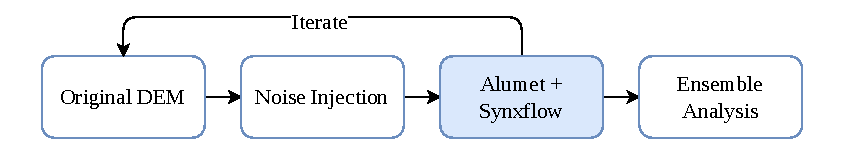
\includegraphics[width=1\textwidth]{images/Workflow.pdf}
  \caption{Computational Pipeline Flowchart}
  \label{fig:design}
\end{figure}

\subsection{Mathematical Formulation}
\label{sec:math}

\begin{itemize}
  \item The artificial topographical noise, which simulates uncertainty, is modeled using a Gaussian probability density function ~\eqref{eq:pdf}.
  \item The mean error is set to zero ($\mu = 0$), assuming that the surveying equipment has no systematic directional bias.
  \item $\sigma$ is the variable controlling the intensity of the simulated sensor noise. The specific discrete levels tested in ensembles are: $\sigma \in \{0.05, 0.1, 0.2, 0.5, 1.0\}$ meters.
  \item The generated noise matrix, defined by $\mathcal{N}(0, \sigma^2)$, is added cell-by-cell to the original DEM elevation matrix to generate the equiprobable realizations.
\end{itemize}

\begin{equation}
f(x) = \frac{1}{\sigma\sqrt{2\pi}} \exp\left(-\frac{(x - \mu)^2}{2\sigma^2}\right)
\label{eq:pdf}
\end{equation}

\subsection{Implementation}
\label{sec:implementation}

\begin{itemize}
  \item All parameters such as boundary conditions, landcover friction values, and temporal settings for the solver are exported from a YAML configuration file to ensure easier experiment reproducibility. 
  \item Synxflow solver is executed as a subprocess wrapped by Alumet. The unique process ID (PID) is identified and extracted from the terminal log file, enabling the isolation of the energy.
  \item Since the energy counters on the CPU and GPU hardware are asynchronous, the post-processing algorithm uses interpolation to match the energy telemetry to a unified timeline.
  \item The Quantity of Interest (QoI) water depth at a specific location is sampled for each iteration. The energy consumption for each iteration is calculated based on the interpolated energy telemetry.
  \item The resulting variance and uncertainty are represented visually using Kernel Density Estimation (KDE) using scipy.stats and matplotlib.
\end{itemize}
  \chapter{Evaluation and Experimental Results}
\label{ch:evaluation}

% Introductory paragraph linking studies to Research Questions (RQs)

\section{Study 0: Single-Run Characterization and Code-Phase Profiling}
\label{sec:res-study0}

Before scaling the framework up to execute full UQ ensembles, it is necessary to validate Alumet's ability to accurately isolate and profile the energy consumption of a single simulation run. Because SynxFlow relies on a heterogeneous execution model, its energy draw varies dynamically between the  CPU and the GPU depending on the active computational phase.

The attributed GPU and CPU time-series plots were generated using the \texttt{alumet-insight} post-processing utility \cite{Correa2026AlumetInsight}.

By correlating the time-series telemetry gathered by Alumet with the cumulative energy curve, the execution pipeline of a single run can be decomposed into two distinct operational phases.

\subsubsection{Phase 1: CPU-Bound Initialization and I/O ($0.0\,\text{s} - 1.0\,\text{s}$)}

The simulation begins with a setup phase bound entirely to the host CPU. As shown in Figure~\ref{fig:study0-cpu}, the CPU telemetry exhibits two distinct power spikes within the first second of execution, while the GPU remains idle near zero active process power. Correlating these spikes with the codebase reveals their reasons. The initial spike corresponds to data ingestion and spatial mapping, where configuration files are parsed, the DEM is loaded into memory via the \texttt{IO.Raster} module, and boundary condition arrays are defined. The second spike corresponds to file compilation, where executing \texttt{case\_input.write\_input\_files()} finalizes environmental matrices and writes the target simulation files to disk.

\begin{figure}[htbp]
    \centering
    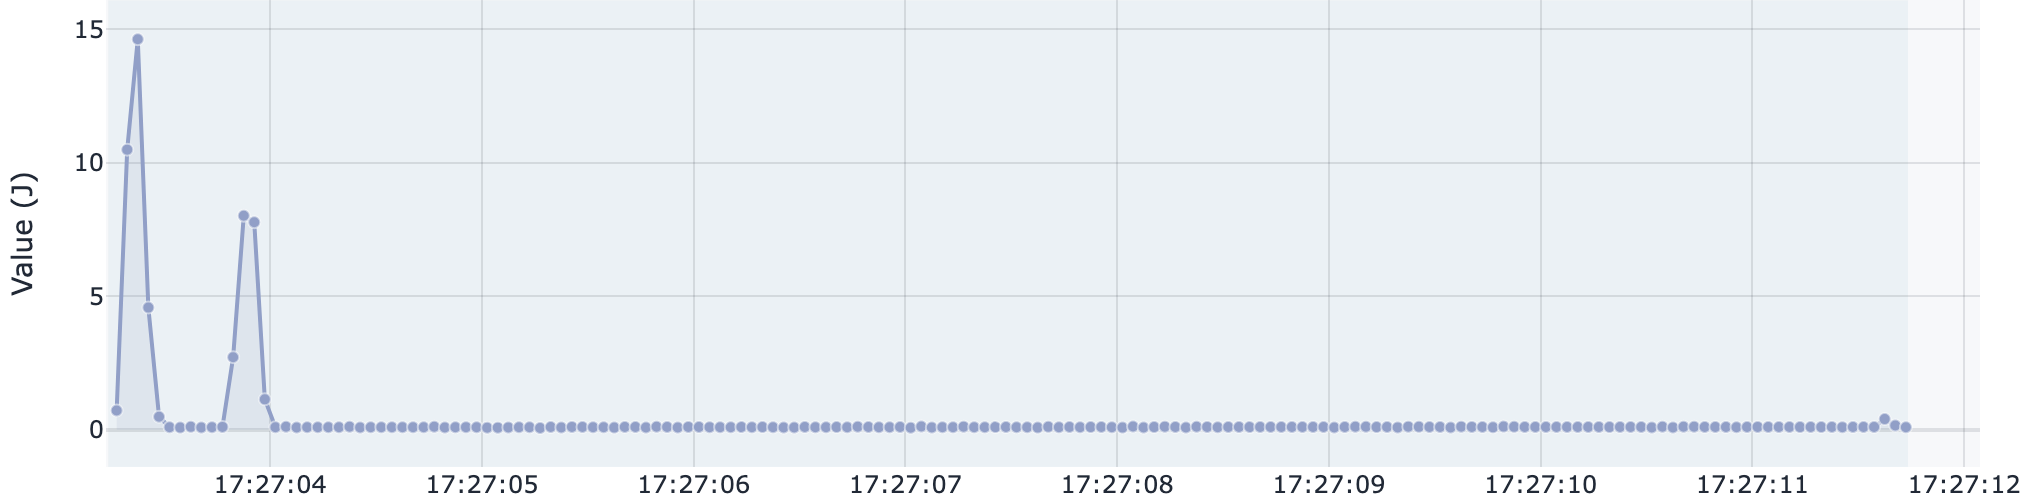
\includegraphics[width=1\textwidth]{images/results/study-0/CPU_energy_timeseries.png}
    \caption{Process-attributed CPU energy time series during single-run execution. Generated using \texttt{alumet-insight} \cite{Correa2026AlumetInsight}.}
    \label{fig:study0-cpu}
\end{figure}

As reflected on the cumulative energy curve (Figure~\ref{fig:study0-cumulative}), these two I/O operations create a discrete stair step accumulation of approximately $50\,\text{J}$ before the solving begins.

\subsubsection{Phase 2: GPU-Bound Solver Execution ($3.0\,\text{s} - 8.5\,\text{s}$)}
Following an idle memory transfer window ($1.0\,\text{s} - 2.7\,\text{s}$), the execution paradigm shifts. CPU power consumption drops to near zero as the process waits on CUDA kernel execution. Simultaneously, the GPU telemetry (Figure~\ref{fig:study0-gpu}) exhibits a sharp power ramp, maintaining sustained power draw throughout the remainder of the iteration.

\begin{figure}[htbp]
    \centering
    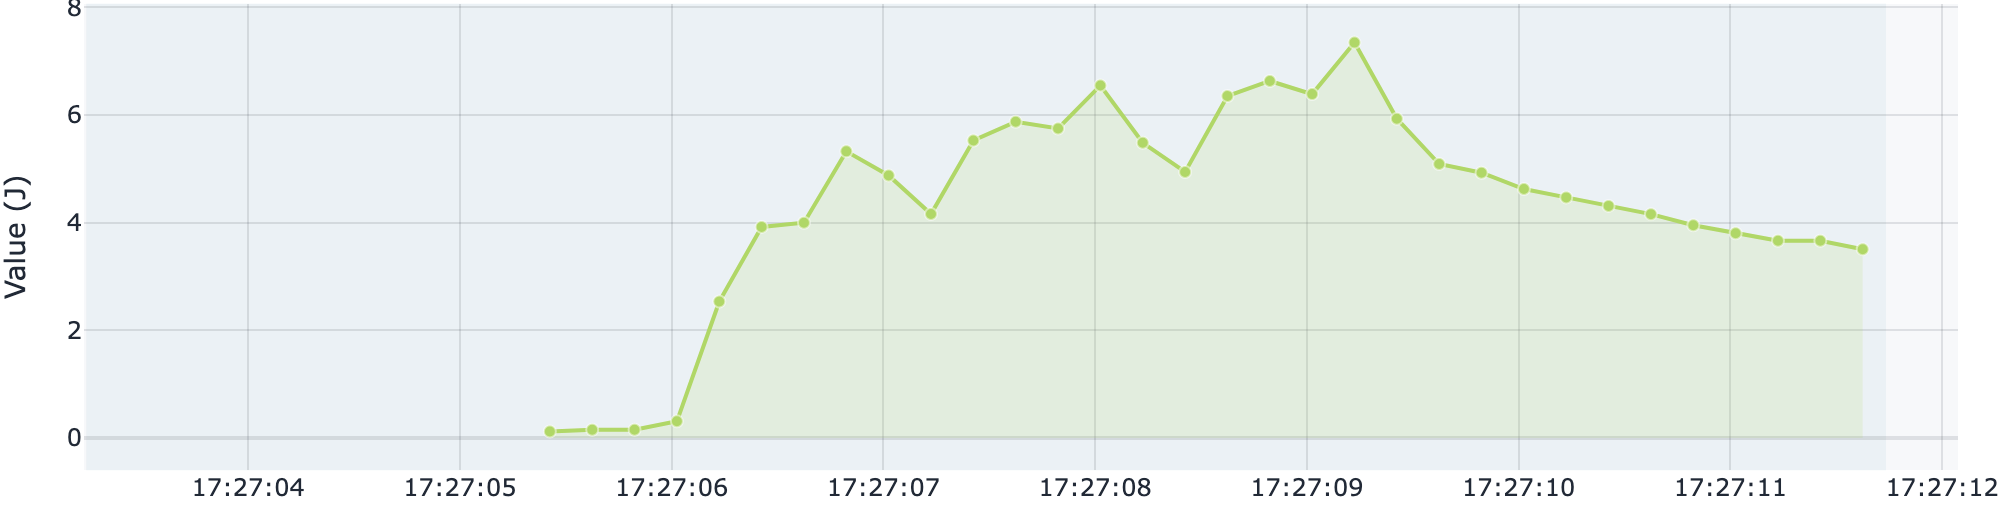
\includegraphics[width=1\textwidth]{images/results/study-0/GPU_energy_timeseries.png}
    \caption{Process-attributed GPU energy time series during single-run execution. Generated using \texttt{alumet-insight} \cite{Correa2026AlumetInsight}.}
    \label{fig:study0-gpu}
\end{figure}

This phase corresponds directly to the dispatch of the \texttt{flood.run()} solver command, where the 2D shallow-water equations are offloaded to CUDA-enabled GPUs for massively parallel processing. On the cumulative timeline (Figure~\ref{fig:study0-cumulative}), this shows as a constant almost linear slope, driving the total single-run energy cost to approximately $205\,\text{J}$.

\begin{figure}[htbp]
    \centering
    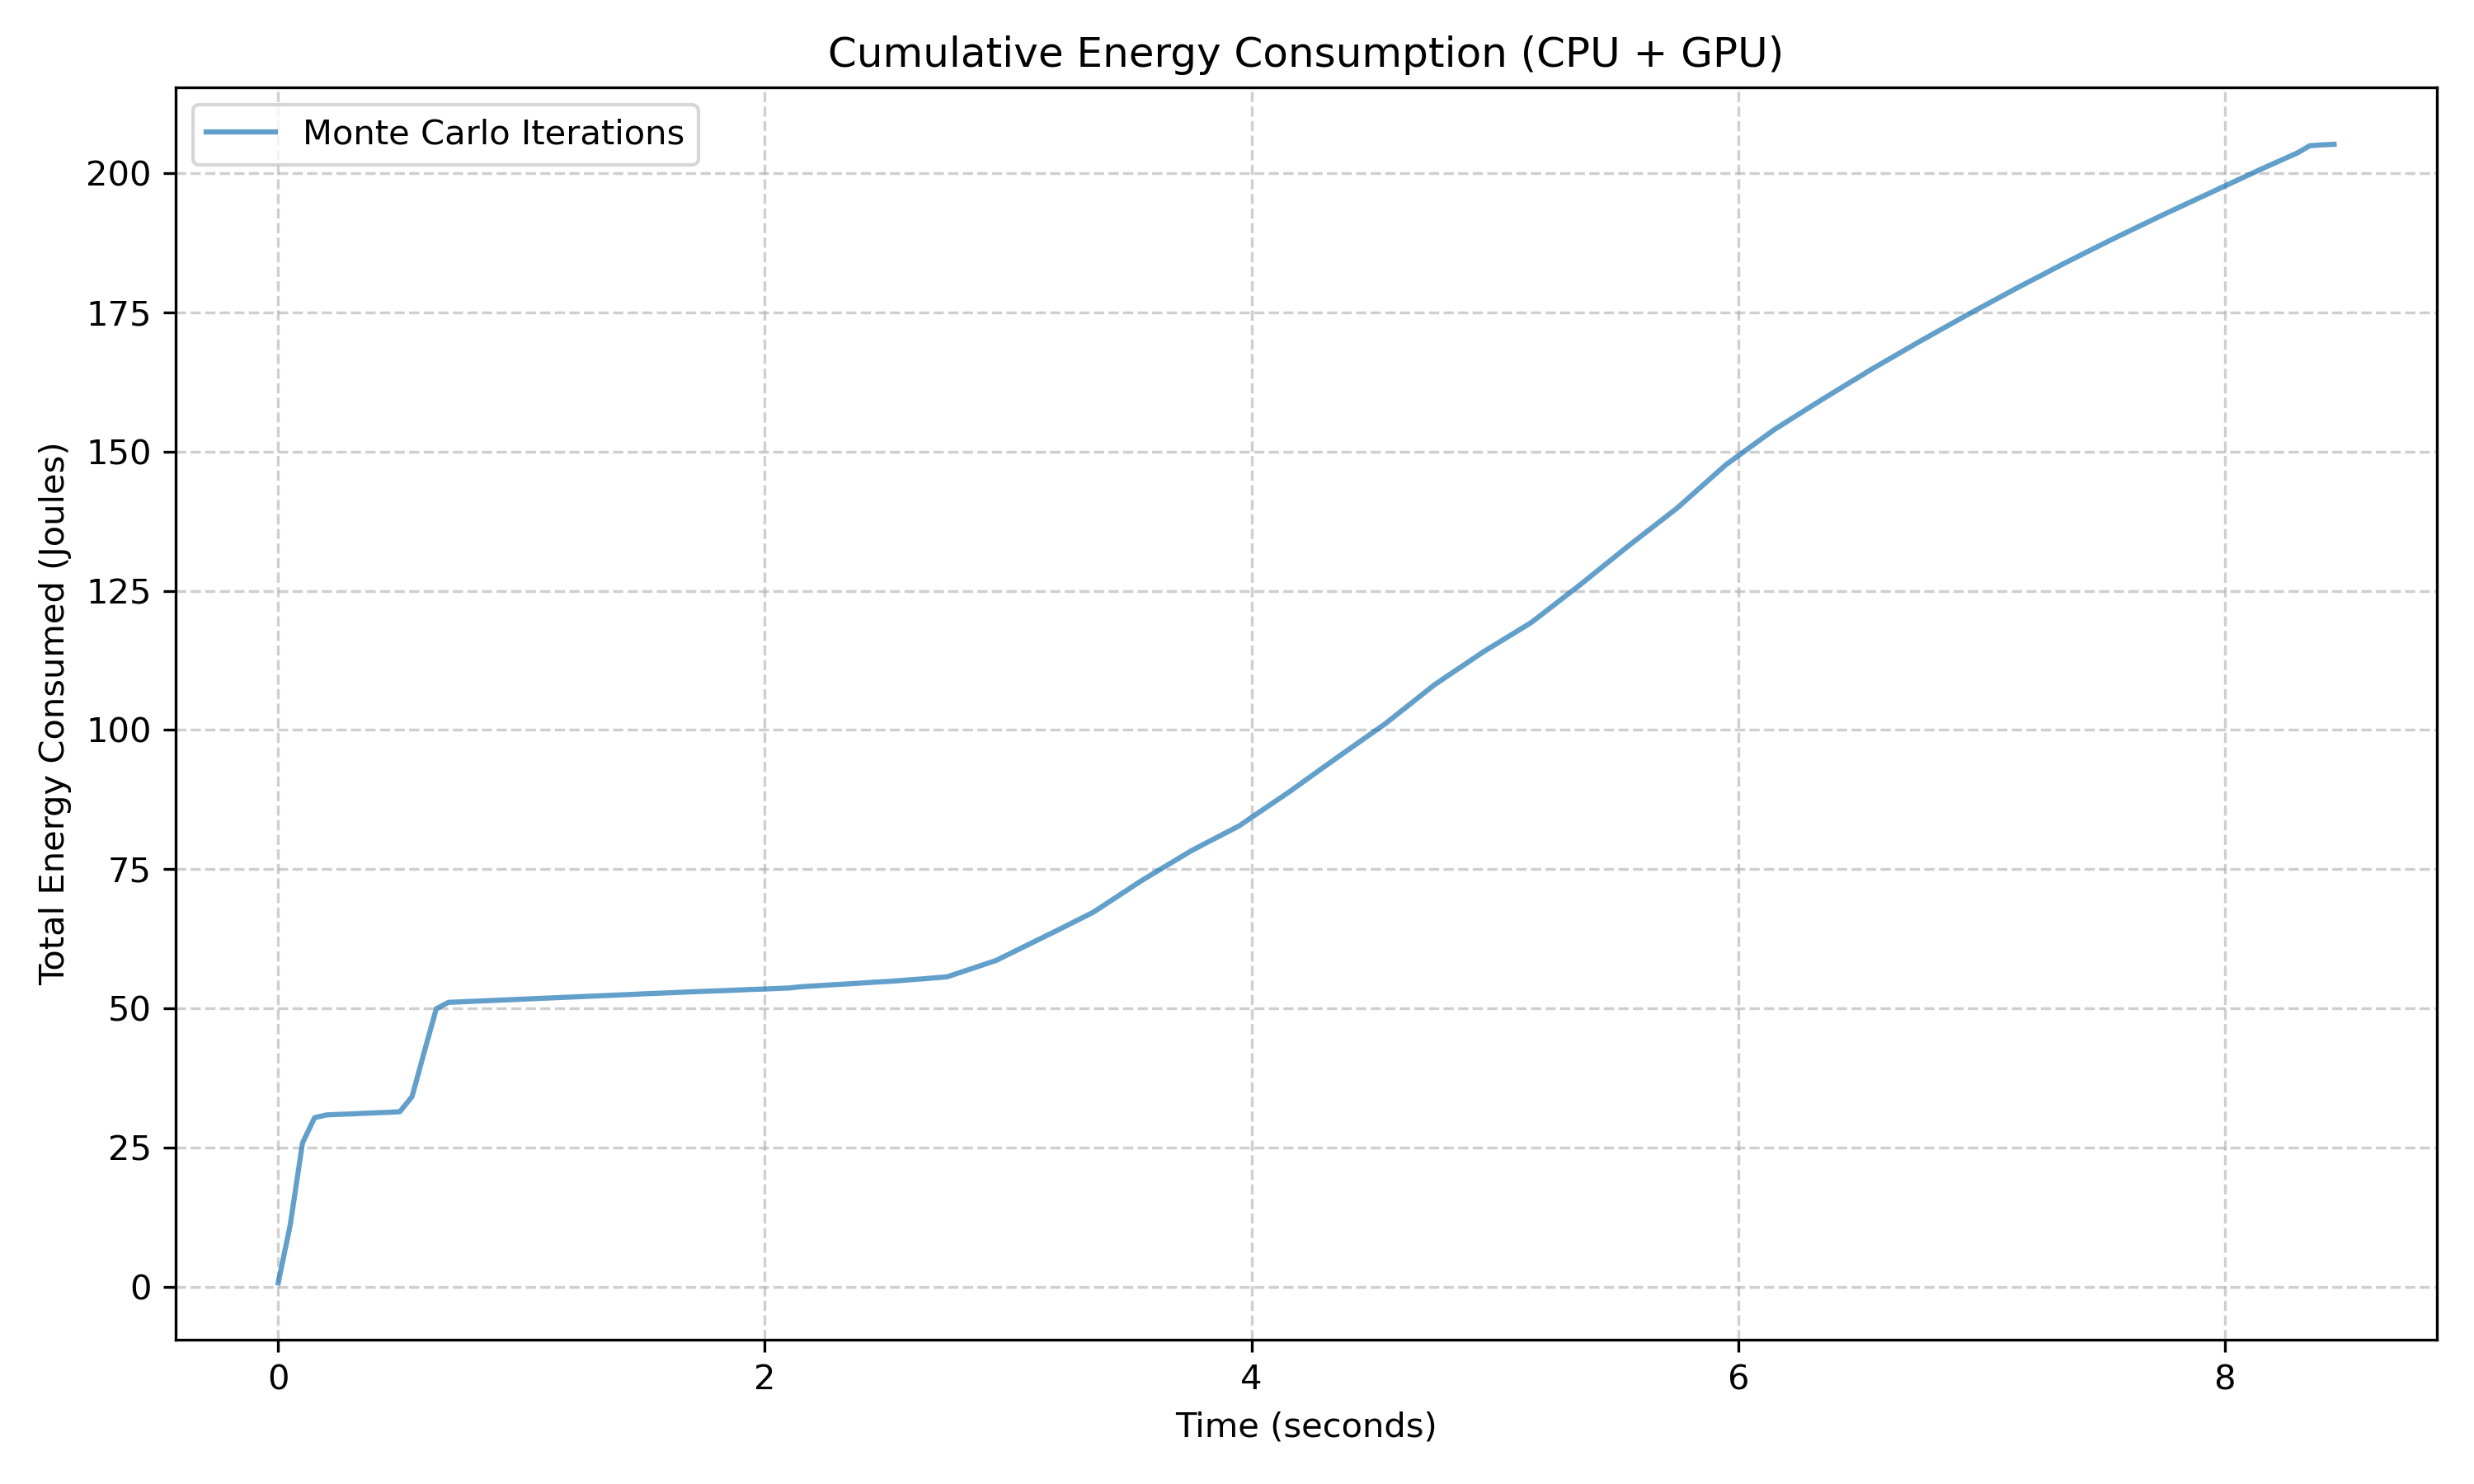
\includegraphics[width=1\textwidth]{images/results/study-0/single_run_cum_energy.png}
    \caption{Cumulative energy timeline (CPU + GPU) for a single simulation run.}
    \label{fig:study0-cumulative}
\end{figure}


\subsection{Results of Study 0}
The observed behavior of the energy curves closely matches the expected execution sequence of the codebase. Therefore these results suggest that the Alumet agent, combined with the dynamic PID-tracking methodology, successfully isolates process-attributed energy across heterogeneous hardware. 

Demonstrating that the framework can distinguish CPU setup spikes from continuous GPU solver draw provides confidence in the methodology, validating the approach to scale up to the large-scale Monte Carlo ensemble in the subsequent studies.

%%%%%%%%%%%%%%%%%%%%%%%%%%%%%%%%%%%%%%%%%%%%%%%%%%%%%%%%%%%%%%%%%%%%%%%%%

\section{Study 1: Evaluation of the Time-to-Solution Energy Proxy}
\label{sec:res-study1}

To address the widespread reliance on execution time as a proxy for energy consumption (as highlighted in Section~\ref{sec:motivation}), this study evaluates whether wall-clock duration reliably predicts process-attributed energy draw across varying mesh workloads. Specifically, this experiment addresses Sub-question 2 by assessing the linearity of the time-energy relationship under deterministic ($\sigma = 0.0\,\text{m}$) execution conditions.

\subsection{Experimental Setup}

To systematically vary the computational workload while preserving similar macro-level flood dynamics, the baseline DEM was resampled into three additional spatial resolution tiers: $10.0\,\text{m}$, $12.0\,\text{m}$, $15.0\,\text{m}$, and $20.0\,\text{m}$, as illustrated in Figure~\ref{fig:dem_grid_comparison}. Adjusting the resolution forces the SynxFlow solver to process different grid dimensions, thereby creating distinct execution durations without altering the underlying physical scenario.

\begin{figure}[htbp]
    \centering
    \begin{subfigure}[b]{0.48\linewidth}
        \centering
        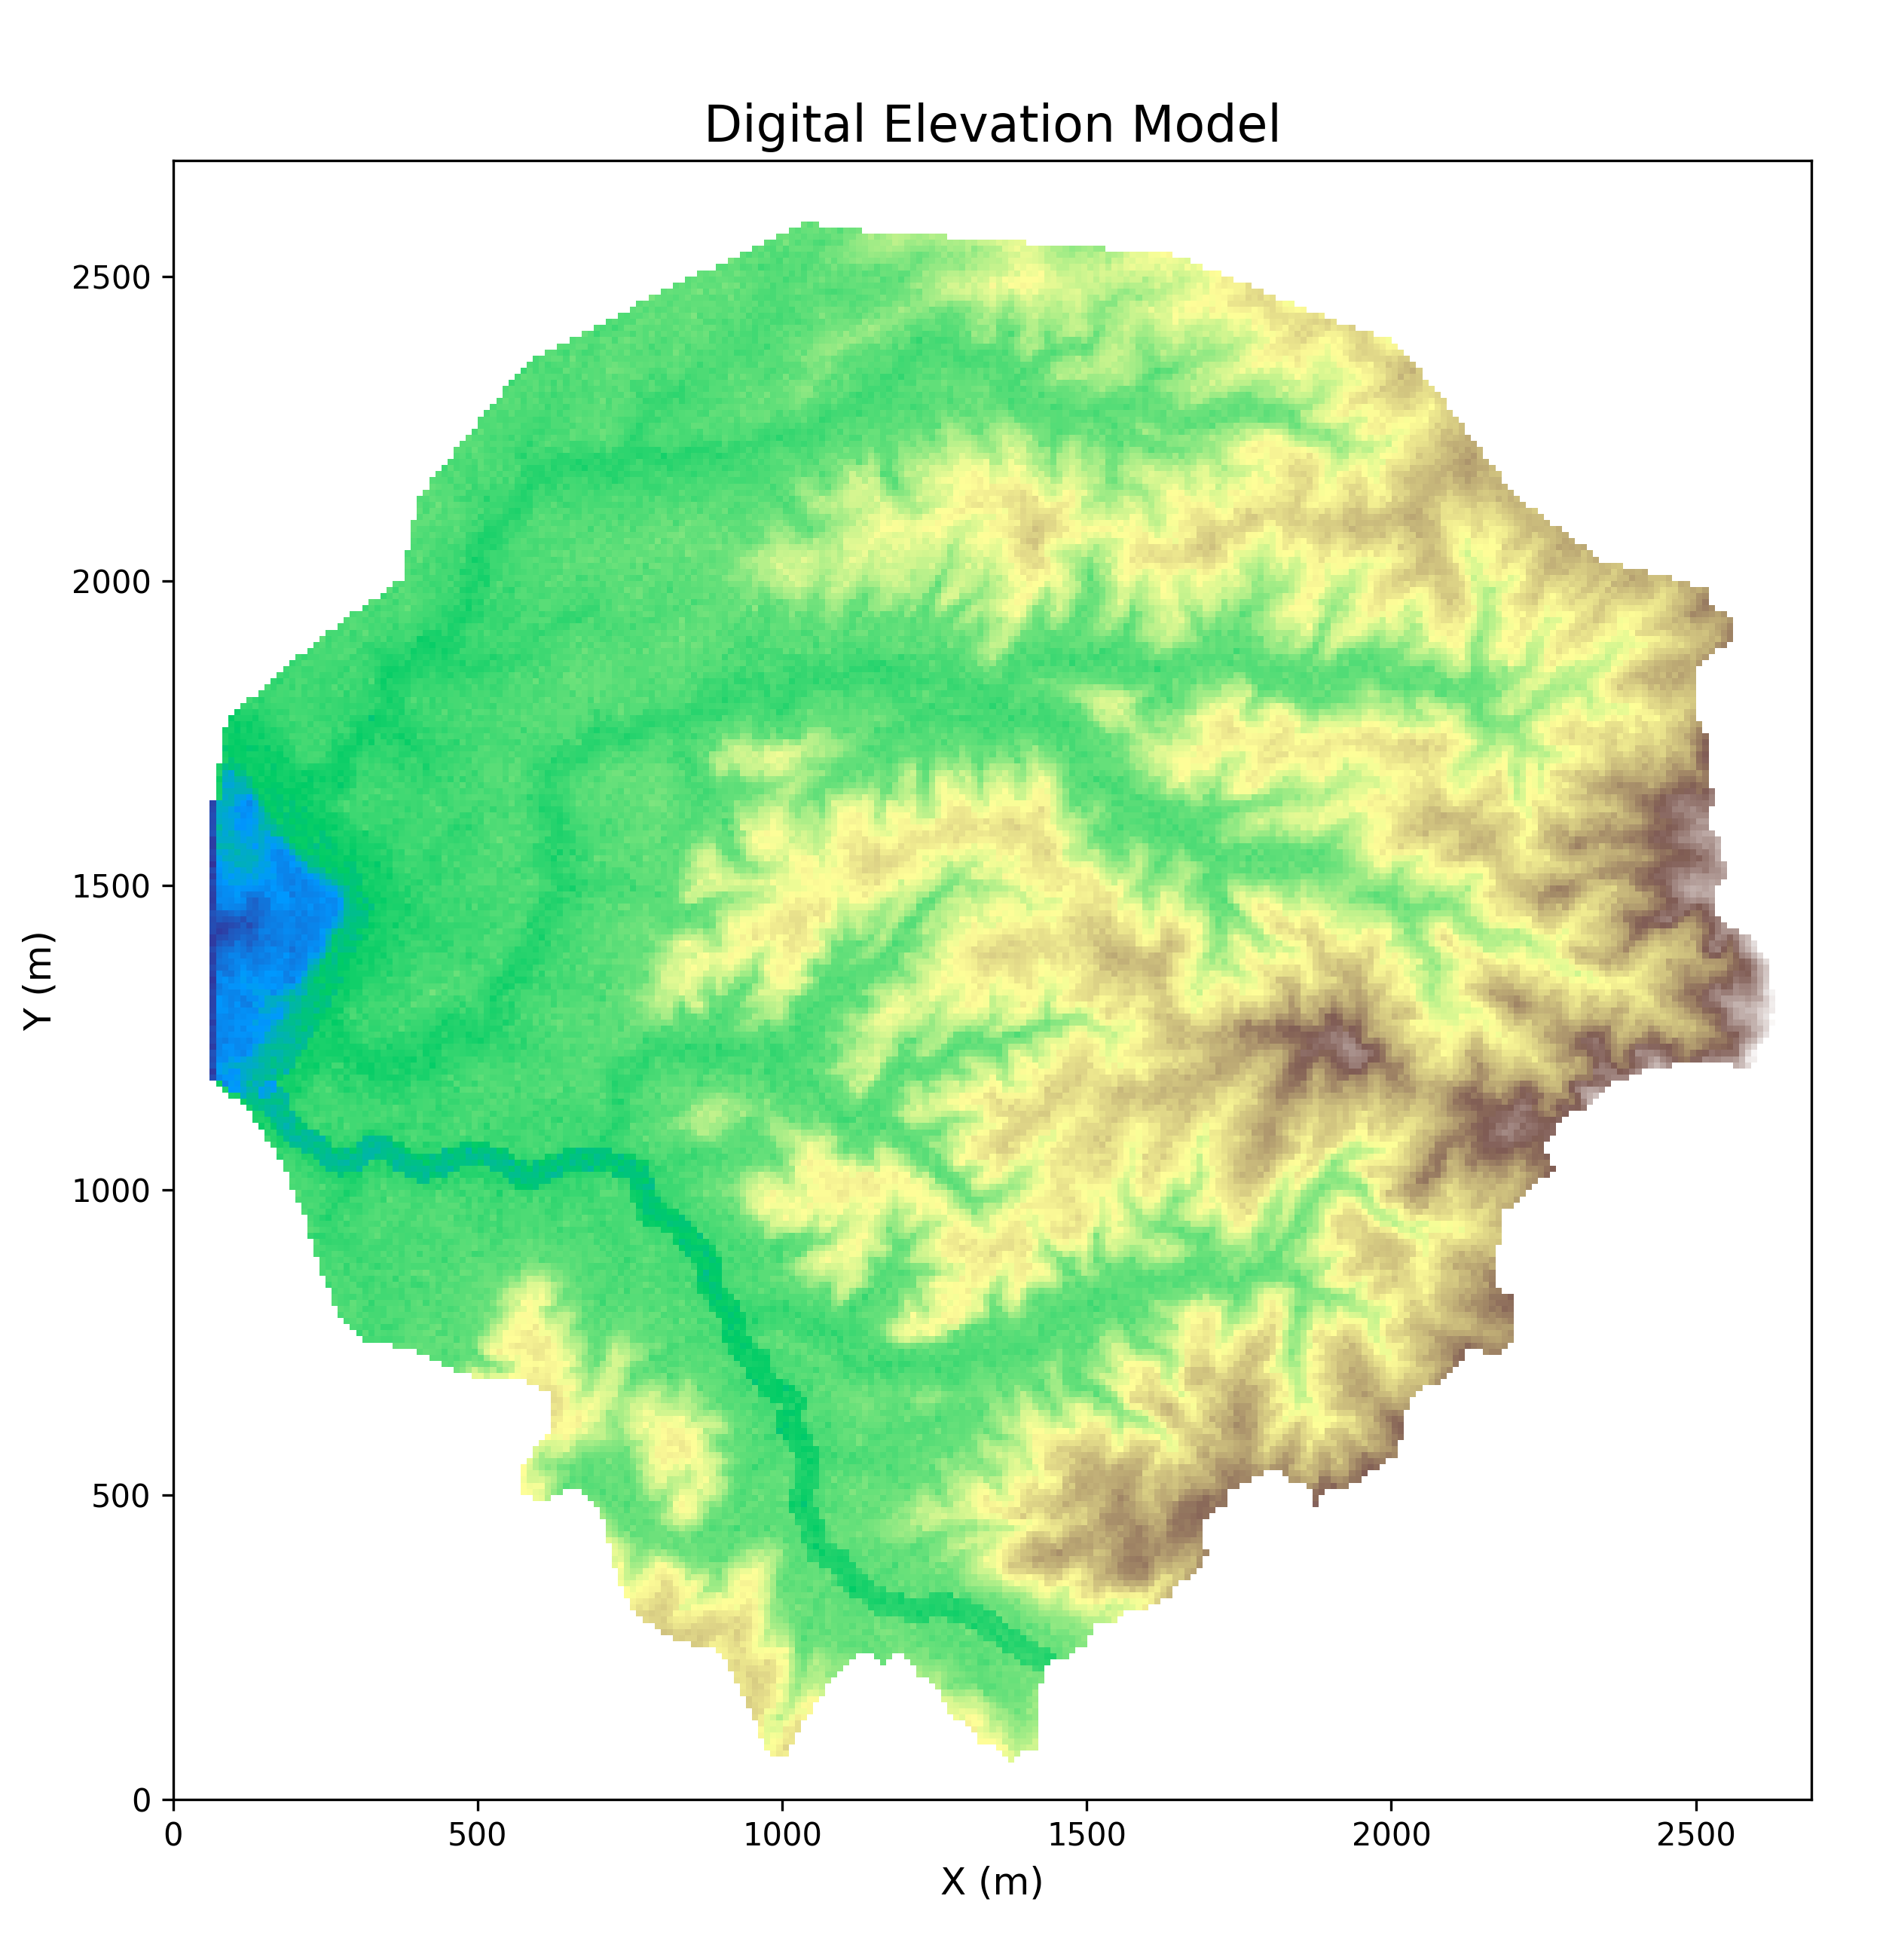
\includegraphics[width=\linewidth]{images/results/time/dem_original.png}
        \caption{Baseline DEM ($10.0\,\text{m}$ resolution).}
        \label{fig:dem_original}
    \end{subfigure}
    \hfill
    \begin{subfigure}[b]{0.48\linewidth}
        \centering
        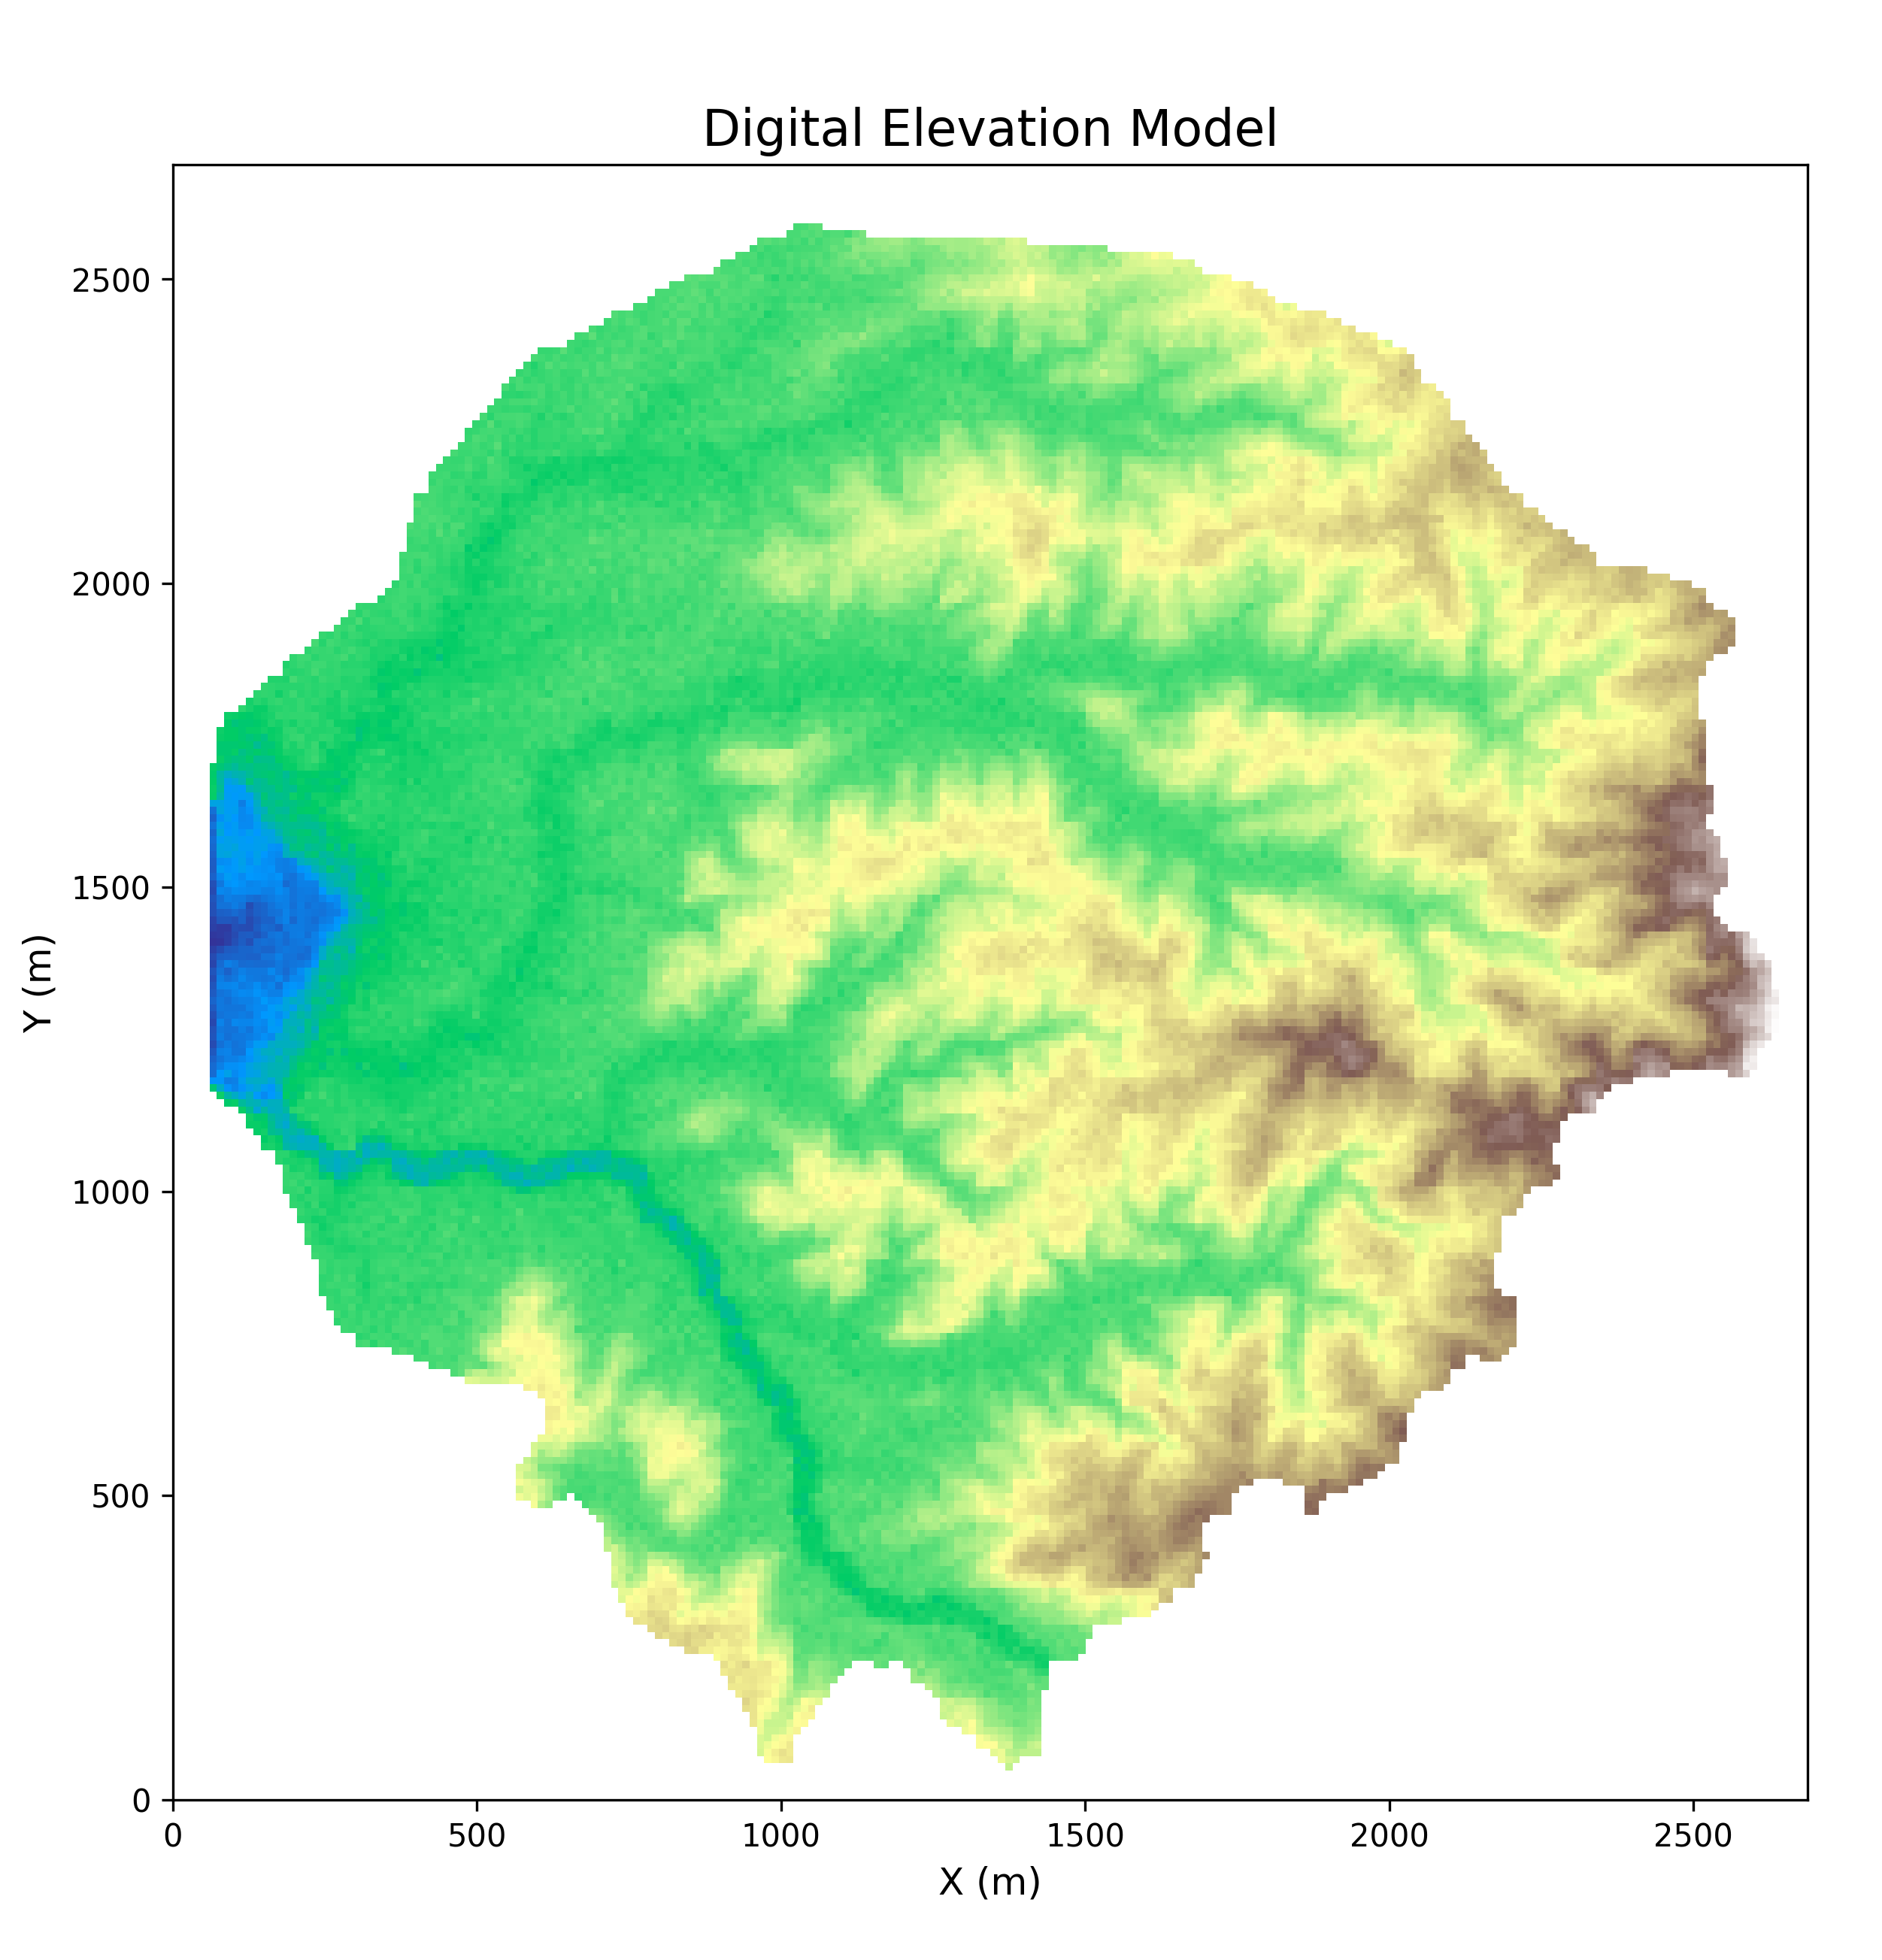
\includegraphics[width=\linewidth]{images/results/time/dem_lowres1.png}
        \caption{Resampled DEM ($12.0\,\text{m}$ resolution).}
        \label{fig:dem_lowres1}
    \end{subfigure}

    \vspace{0.8em}

    \begin{subfigure}[b]{0.48\linewidth}
        \centering
        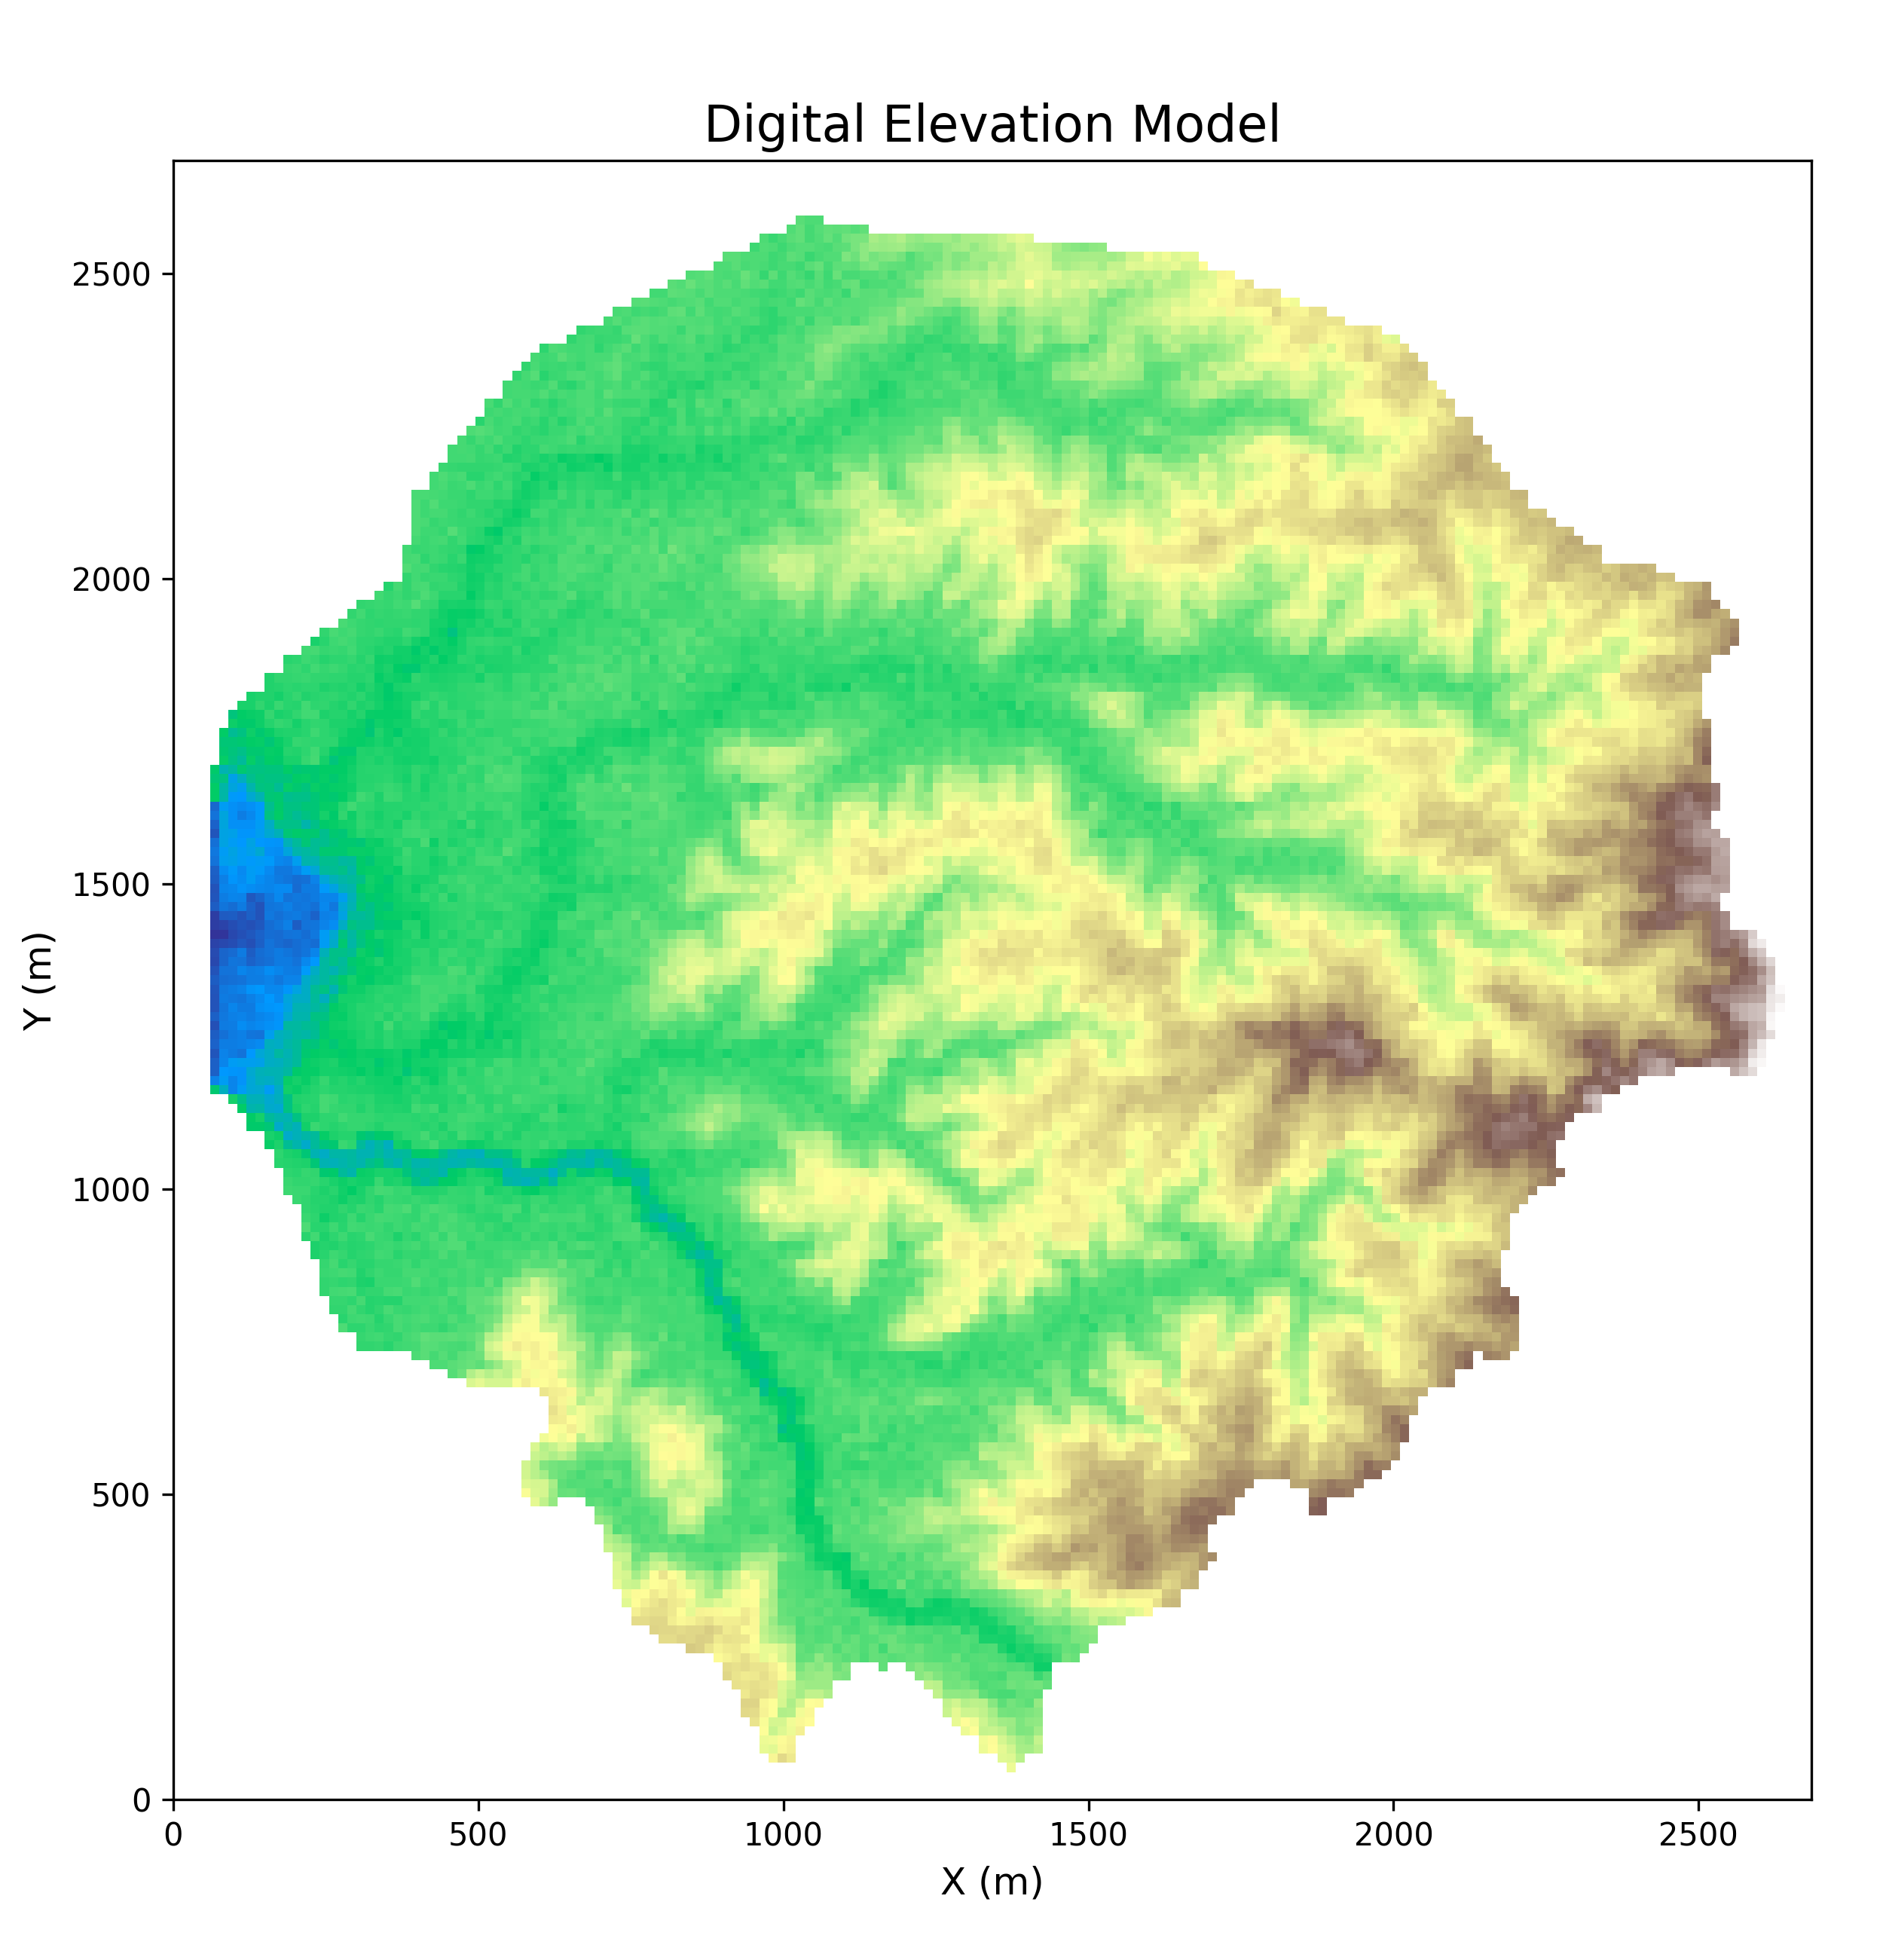
\includegraphics[width=\linewidth]{images/results/time/dem_lowres2.png}
        \caption{Resampled DEM ($15.0\,\text{m}$ resolution).}
        \label{fig:dem_lowres2}
    \end{subfigure}
    \hfill
    \begin{subfigure}[b]{0.48\linewidth}
        \centering
        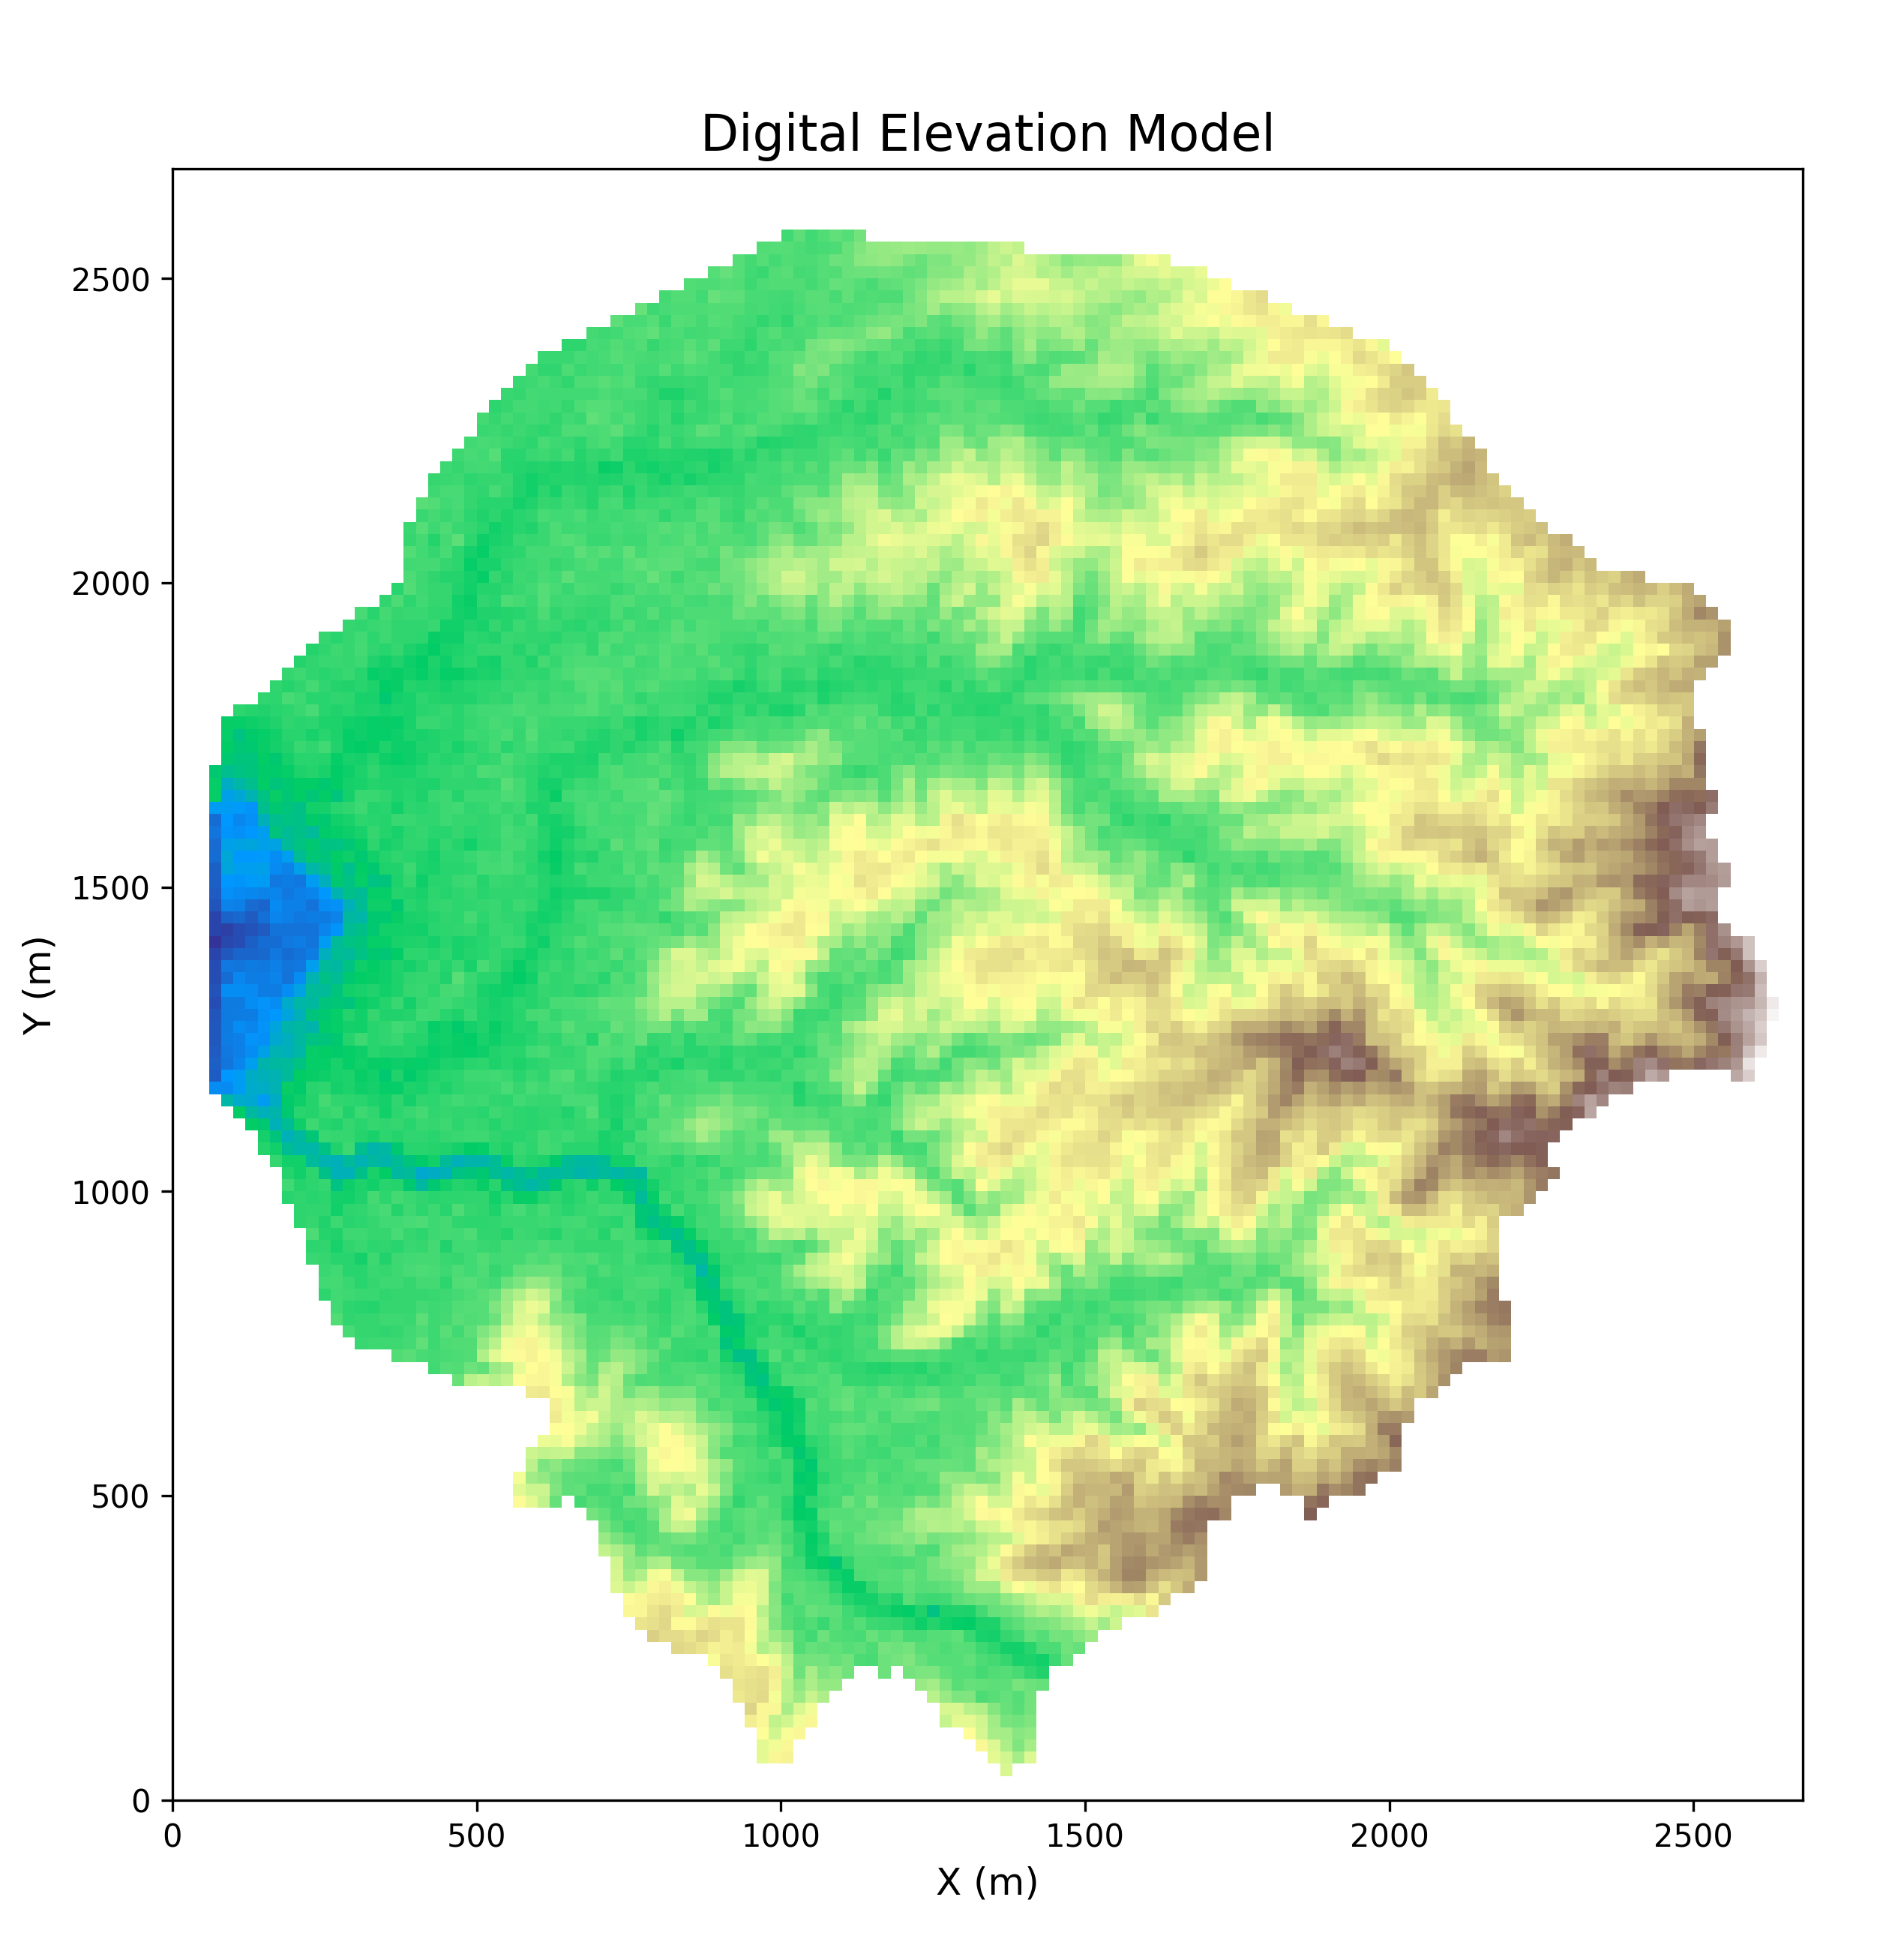
\includegraphics[width=\linewidth]{images/results/time/dem_lowres3.png}
        \caption{Resampled DEM ($20.0\,\text{m}$ resolution).}
        \label{fig:dem_lowres3}
    \end{subfigure}

    \caption{Grid comparison of the DEM resampled across four resolutions to alter solver execution workloads.}
    \label{fig:dem_grid_comparison}
\end{figure}

For each DEM resolution, an ensemble of 100 iterations was executed with the topographic noise strictly set to zero ($\sigma = 0.0\,\text{m}$). Setting the input noise to zero holds the physical elevation raster completely identical across all 100 iterations of a given resolution. In a deterministic computing environment, identical inputs should yield the same execution time and energy consumption. Because the terrain input remains completely constant in this experiment, any observed variability isolates execution uncertainty rather than physical terrain noise.

\subsection{Statistical Framework and Metrics}

To accurately reflect the dynamic execution environment and evaluate the time-proxy relationship across the resolution ensembles, the telemetry data is analyzed using the following statistical framework:

\paragraph{Data Filtration via Z-Scores:}
In shared High-Performance Computing (HPC) environments, random background operating system spikes or node communication delays can cause execution stalls that do not reflect the solver's actual mathematical workload. To isolate the solver's true efficiency, Z-scores are computed for both total execution duration and energy-per-second. Runs exceeding a defined standard deviation threshold (e.g., $Z > 2.0$) are flagged as outliers and removed from the clean dataset. This ensures that the subsequent metrics evaluate the hydrodynamic solver rather than transient cluster traffic.

\paragraph{Mean Average Power:}
For each individual run, the average power draw (in Watts) is extracted by computing the slope of the cumulative energy timeline using an ordinary least squares regression. Calculating the mean ($\mu$) of this power draw across the ensemble establishes the true hardware baseline for each spatial resolution tier.

\paragraph{($R^2$) Coefficient of Determination:}
This metric serves as the primary analytical tool to directly test the time-proxy assumption. Fundamental physical power modeling relies on the relationship:
\begin{equation}
E = A + P \cdot t
\label{eq:energy_power_time}
\end{equation}
where $E$ is total energy, $A$ represents static idle energy overhead, $P$ is dynamic power draw, and $t$ is execution time \cite{Tian2014}.
If time is a perfect proxy for energy, dynamic power ($P$) must remain constant across iterations, meaning execution time and total energy would form a perfectly linear relationship ($R^2 = 1.0$). By running a linear regression across the execution times and total energy costs of the iterations, the framework directly tests this linearity. A reduced $R^2$ value points toward dynamic power fluctuations across runs, which undermines the assumption that execution time can be used as a simple standalone proxy.

\paragraph{Welch's t-test (Independent Samples):}
To determine how varying computational workloads affect underlying hardware behavior, Welch's t-test is applied to compare the average power draw between the different DEM resolution groups. This test determines whether altering the grid dimension causes a statistically significant shift in the rate at which the hardware consumes energy.


\subsection{Results of Study 1}

The telemetry data extracted from the ensembles provides three key observations regarding the validity of using execution time as an energy proxy.

The raw telemetry data highlights potential cluster volatility before statistical filtering is applied. As shown in Figure~\ref{fig:proxy-fallacy}, tracking the total energy against execution duration for all iterations reveals instances of what appear to be execution stalls. While several outlier runs experienced extended durations, jumping from a baseline of under $10\,\text{s}$ to over $60\,\text{s}$, it is important to note that these iterations still yielded valid physical outputs. The exact underlying cause of their extended runtime is not definitively known. However, such delays could plausibly be caused by temporary I/O bottlenecks, background operating system tasks, or resource contention. Because the physical inputs were strictly identical across these iterations, algorithmic variations such as the solver dynamically reducing its timestep are highly unlikely to be the root cause. This is further supported by the disproportionately low power rate of these outliers, which suggests the hardware was idling rather than actively performing computations. Despite the increases in execution time between runs, the corresponding energy draw did not appear to scale proportionally, resulting in a degraded linear fit ($R^2 = 0.165$). This suggests that relying just on wall-clock time as an energy metric may be susceptible to external cluster interference. The Z-score filtering methodology was applied to identify and exclude these longer runs from the dataset to isolate the solver's active computational footprint.

\begin{figure}[H]
    \centering
    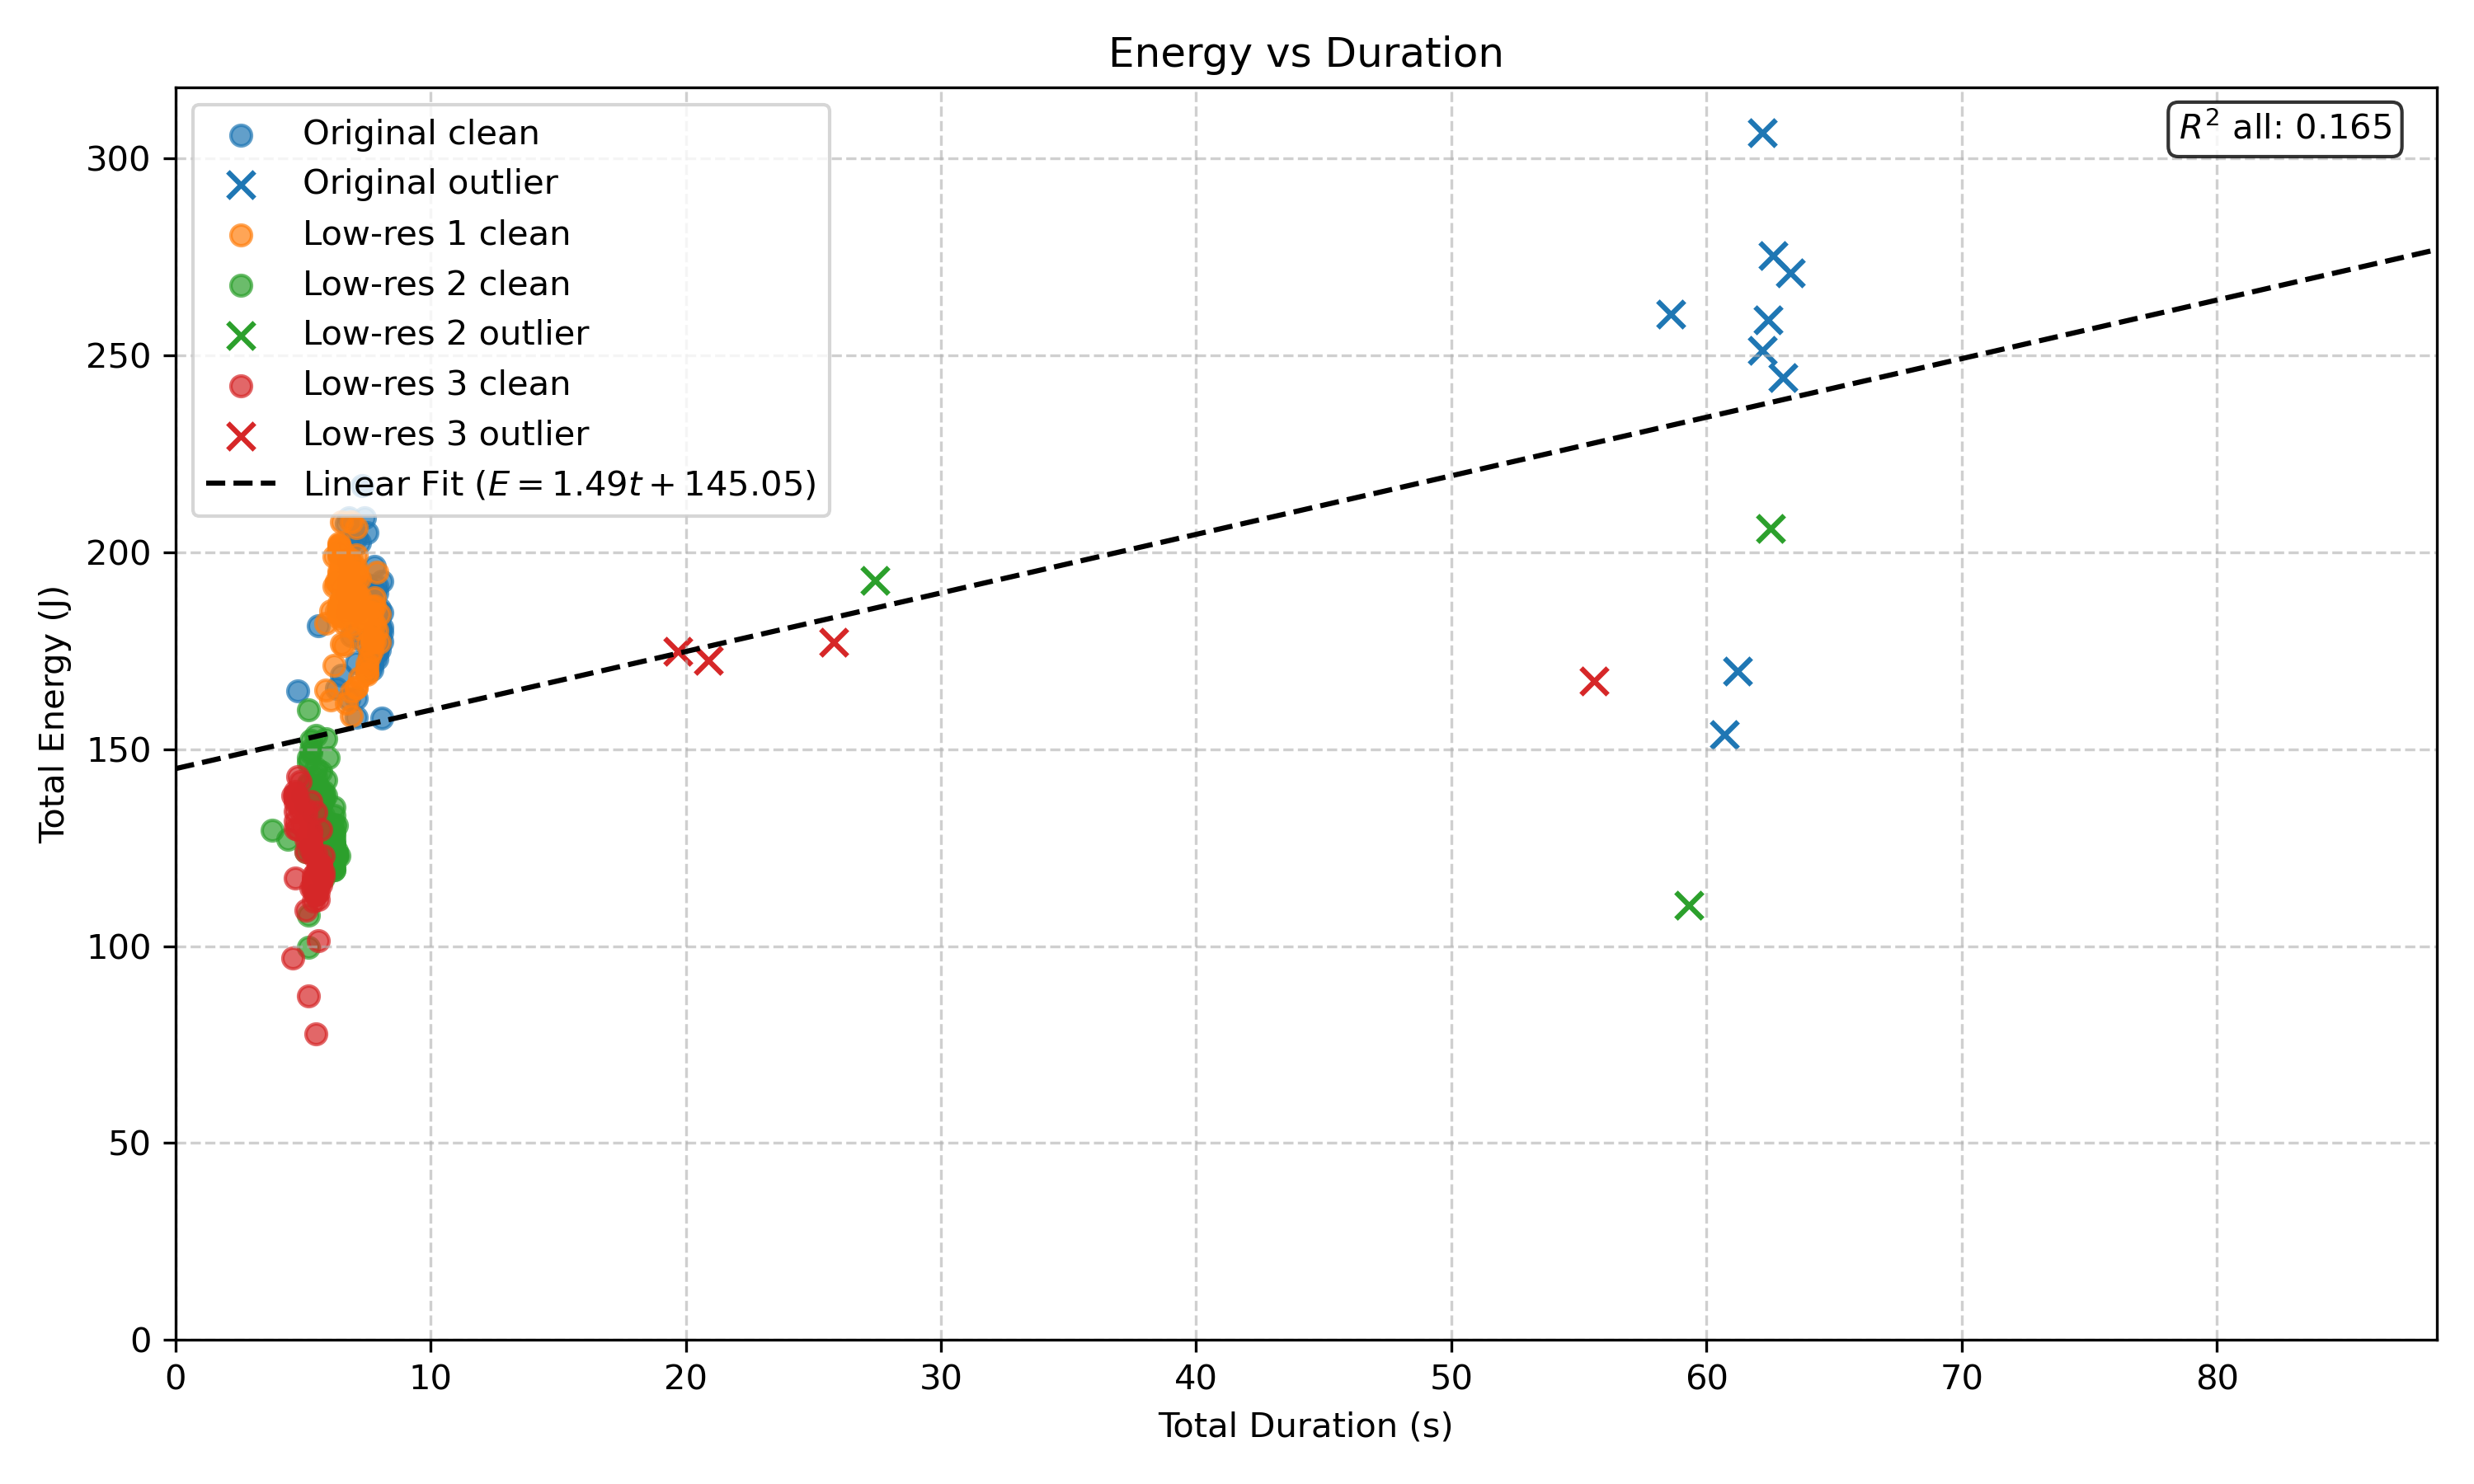
\includegraphics[width=1\textwidth]{images/results/time/proxy_fallacy.png}
    \caption{Total energy consumption vs. execution duration for all iterations.}
    \label{fig:proxy-fallacy}
\end{figure}

After filtering the outliers, the clean dataset was evaluated to test if dynamic power remains constant across iterations. If energy consumption were primarily driven by execution duration, the filtered data would theoretically exhibit a highly linear correlation (near $R^2 = 1.0$). Figure~\ref{fig:proxy-fallacy-clean} reveals that even under clean and stable cluster conditions, this relationship remains surprisingly weak. The linear regression for the clean iterations yields a Coefficient of Determination of $R^2 = 0.518$. A value this low suggests that nearly half of the variance in energy consumption cannot be explained by the execution time alone. This divergence indicates that the solver's hardware usage, and therefore its dynamic power, fluctuates between iterations. Consequently, within the context of this study, time-to-solution appears to be an unreliable standalone proxy for total energy cost.

\begin{figure}[H]
    \centering
    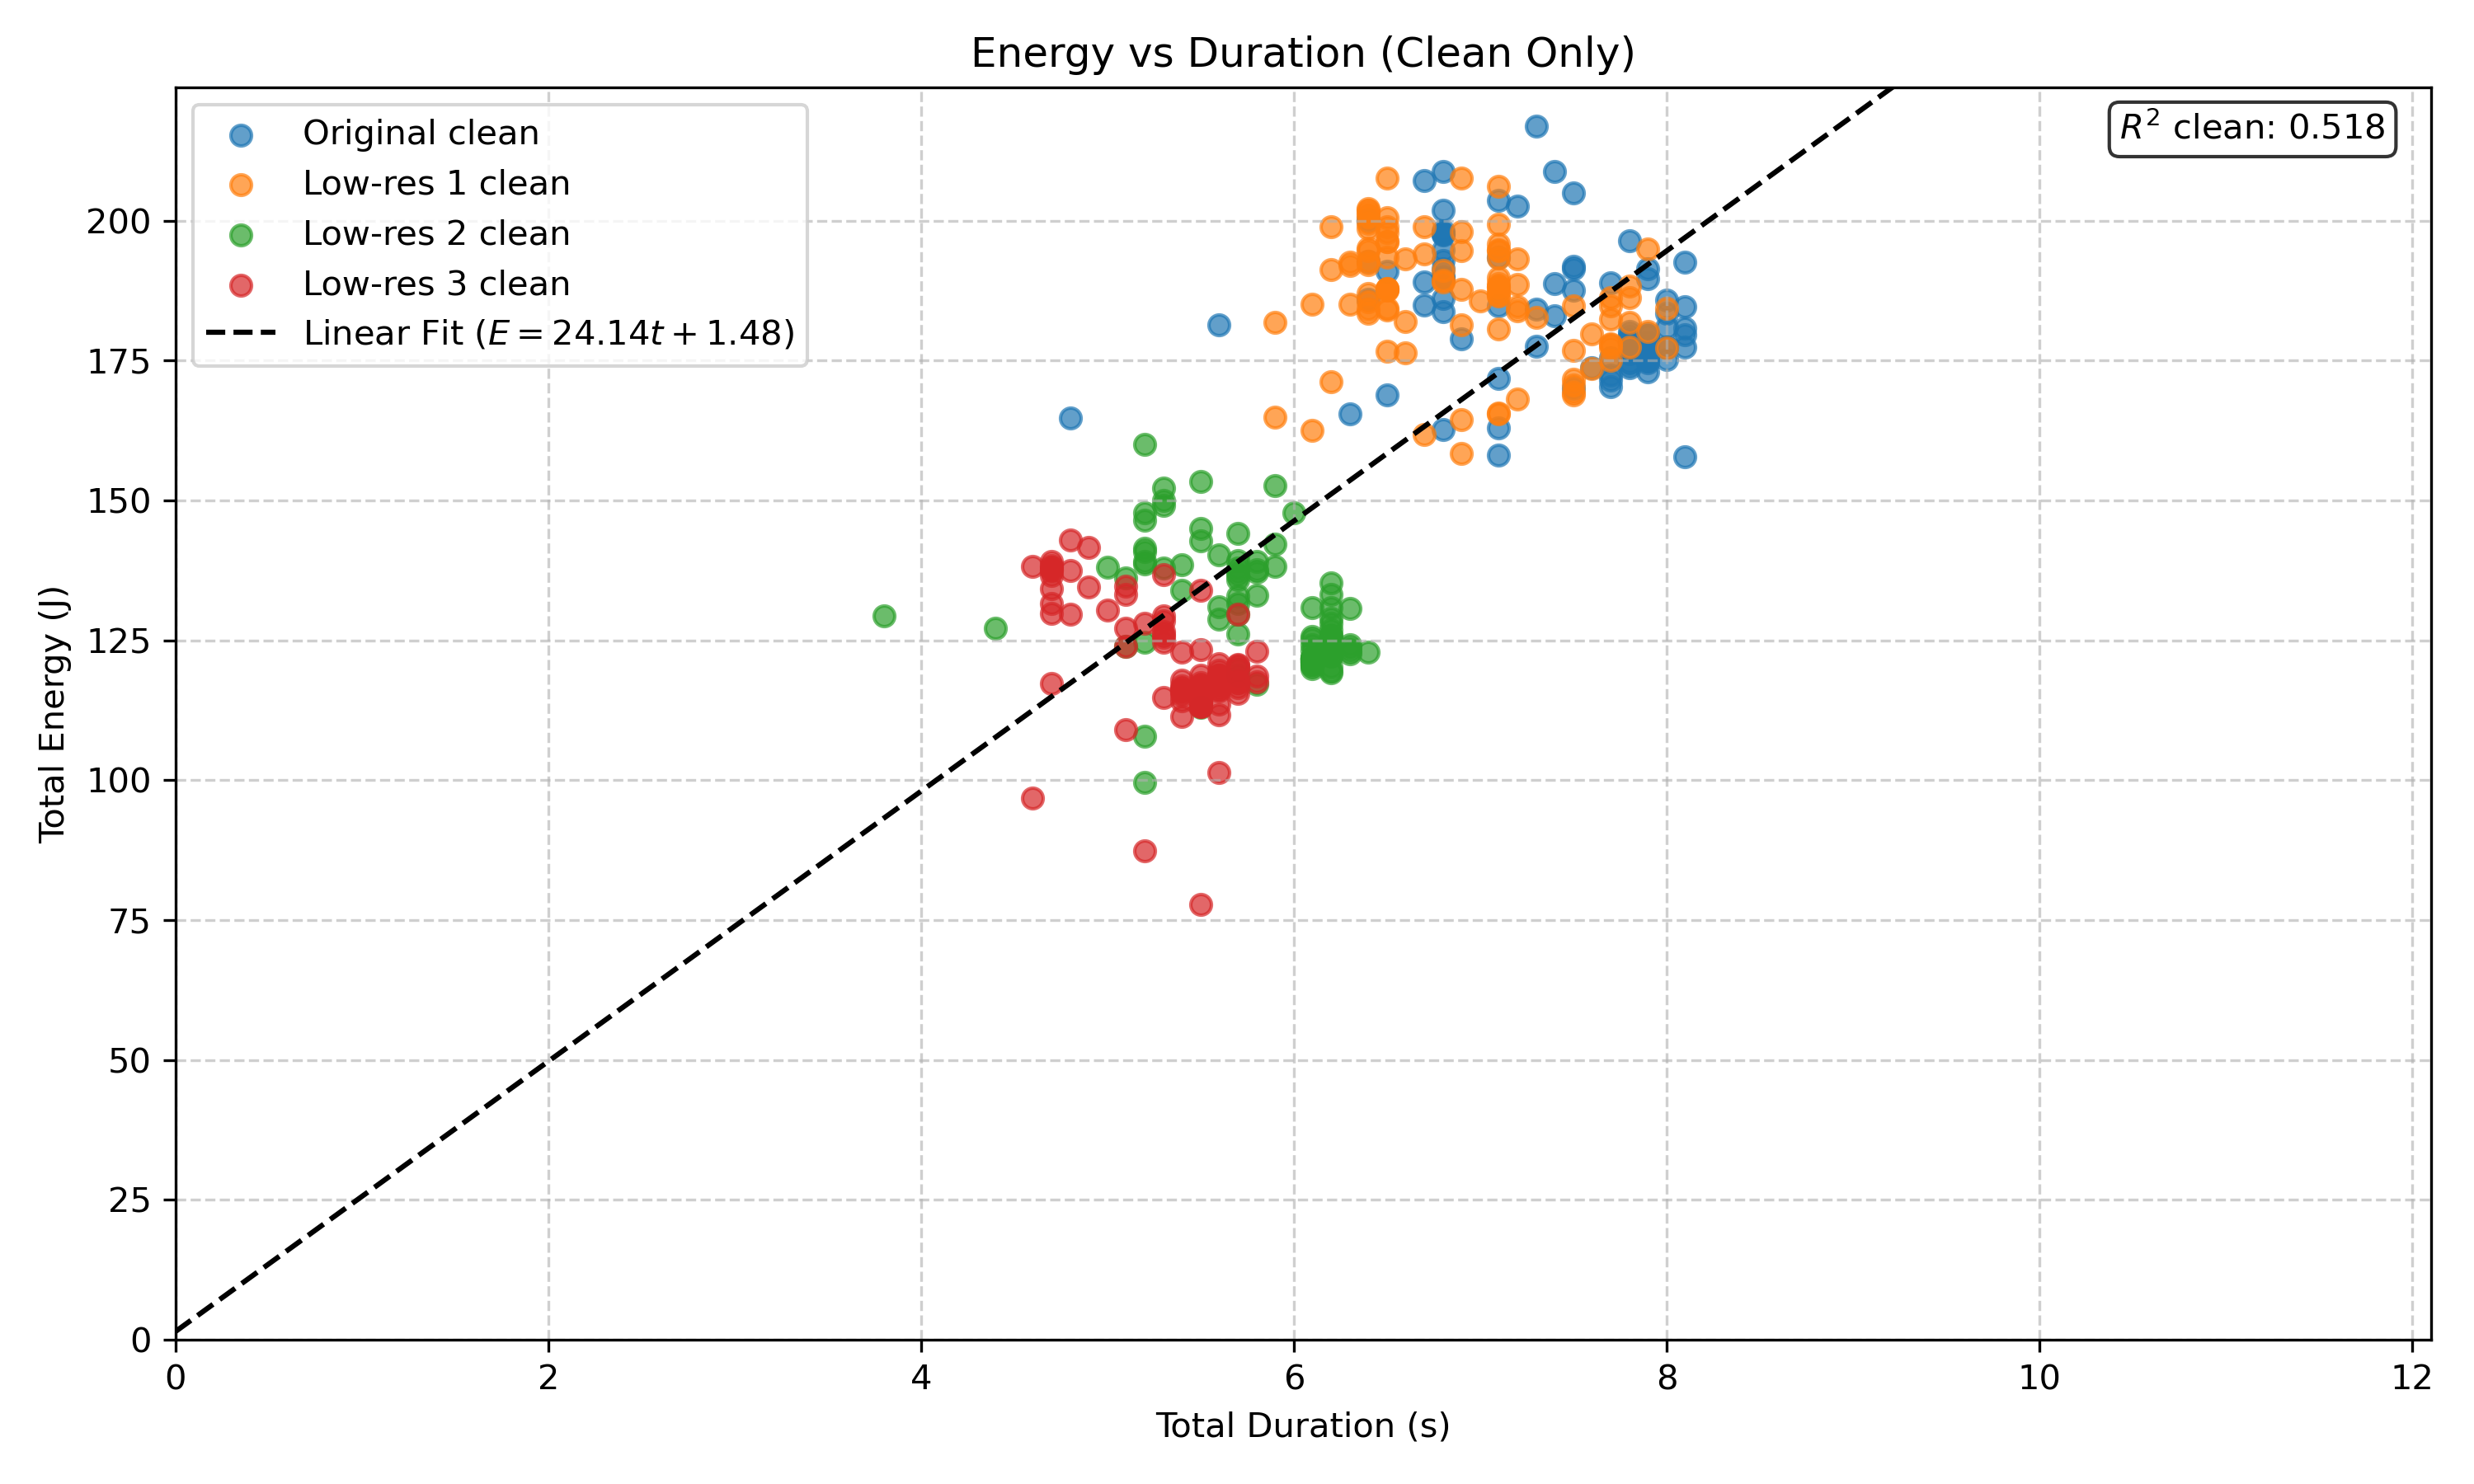
\includegraphics[width=1\textwidth]{images/results/time/proxy_fallacy_clean.png}
    \caption{Total energy consumption vs. execution duration for all clean iterations.}
    \label{fig:proxy-fallacy-clean}
\end{figure}

The underlying cause of this non-linearity is further clarified by examining the average power draw across the different resolution tiers. Figure~\ref{fig:power-signature} plots the average cumulative energy trajectories for each spatial resolution. The slope of these curves represents the dynamic power draw in Watts. The data illustrates that power is not a static constant; it shifts dynamically based on the grid resolution being processed. For example, the $12.0\,\text{m}$ resolution exhibited an average power draw of $22.68\,\text{W}$, while the coarser $15.0\,\text{m}$ and $20.0\,\text{m}$ resolutions operated at lower intensities of $17.14\,\text{W}$ and $16.90\,\text{W}$, respectively.

\begin{table}[htbp]
  \centering
  \begin{tabular}{lccc}
    \toprule
    \textbf{Resolution Comparison} & \textbf{$t$-statistic} & \textbf{$p$-value} & \textbf{Significant ($p < 0.05$)?} \\
    \midrule
    $10.0\,\text{m}$ vs. $12.0\,\text{m}$ & -4.684 & $< 0.001$ & Yes \\
    $10.0\,\text{m}$ vs. $15.0\,\text{m}$ & 12.183 & $< 0.001$ & Yes \\
    $10.0\,\text{m}$ vs. $20.0\,\text{m}$ & 13.457 & $< 0.001$ & Yes \\
    $12.0\,\text{m}$ vs. $15.0\,\text{m}$ & 17.084 & $< 0.001$ & Yes \\
    $12.0\,\text{m}$ vs. $20.0\,\text{m}$ & 18.634 & $< 0.001$ & Yes \\
    $15.0\,\text{m}$ vs. $20.0\,\text{m}$ & 0.743 & 0.458 & No \\
    \bottomrule
  \end{tabular}
  \caption{Welch's t-test results comparing the average power draw between different grid resolution ensembles.}
  \label{tab:welch-ttest}
\end{table}

A Welch's t-test confirms that these shifts in hardware intensity are statistically significant ($p < 0.001$) across almost all workload transitions. The test also highlights an unexpected dynamic: the $12.0\,\text{m}$ resolution draws a significantly higher average power than the more complex $10.0\,\text{m}$ baseline ($t = -4.684$, $p < 0.001$). This suggests that a higher power draw may not strictly indicate a larger total mathematical workload, but could instead reflect higher hardware utilization efficiency. It is plausible that the array dimensions of the $12.0\,\text{m}$ grid align more optimally with the GPU's cache limits or thread block architecture. This alignment would decrease memory stalls, allowing the processing cores to operate at a higher, more continuous intensity per second despite having fewer total cells to compute. Conversely, the comparison between the two coarsest grids ($15.0\,\text{m}$ and $20.0\,\text{m}$) yielded no statistically significant difference in power draw ($t = 0.743$, $p = 0.458$). This implies that while grid resolution and hardware alignment actively influence dynamic power, the system's power usage might stabilize once the computational grid becomes sufficiently sparse.

\begin{figure}[H]
    \centering
    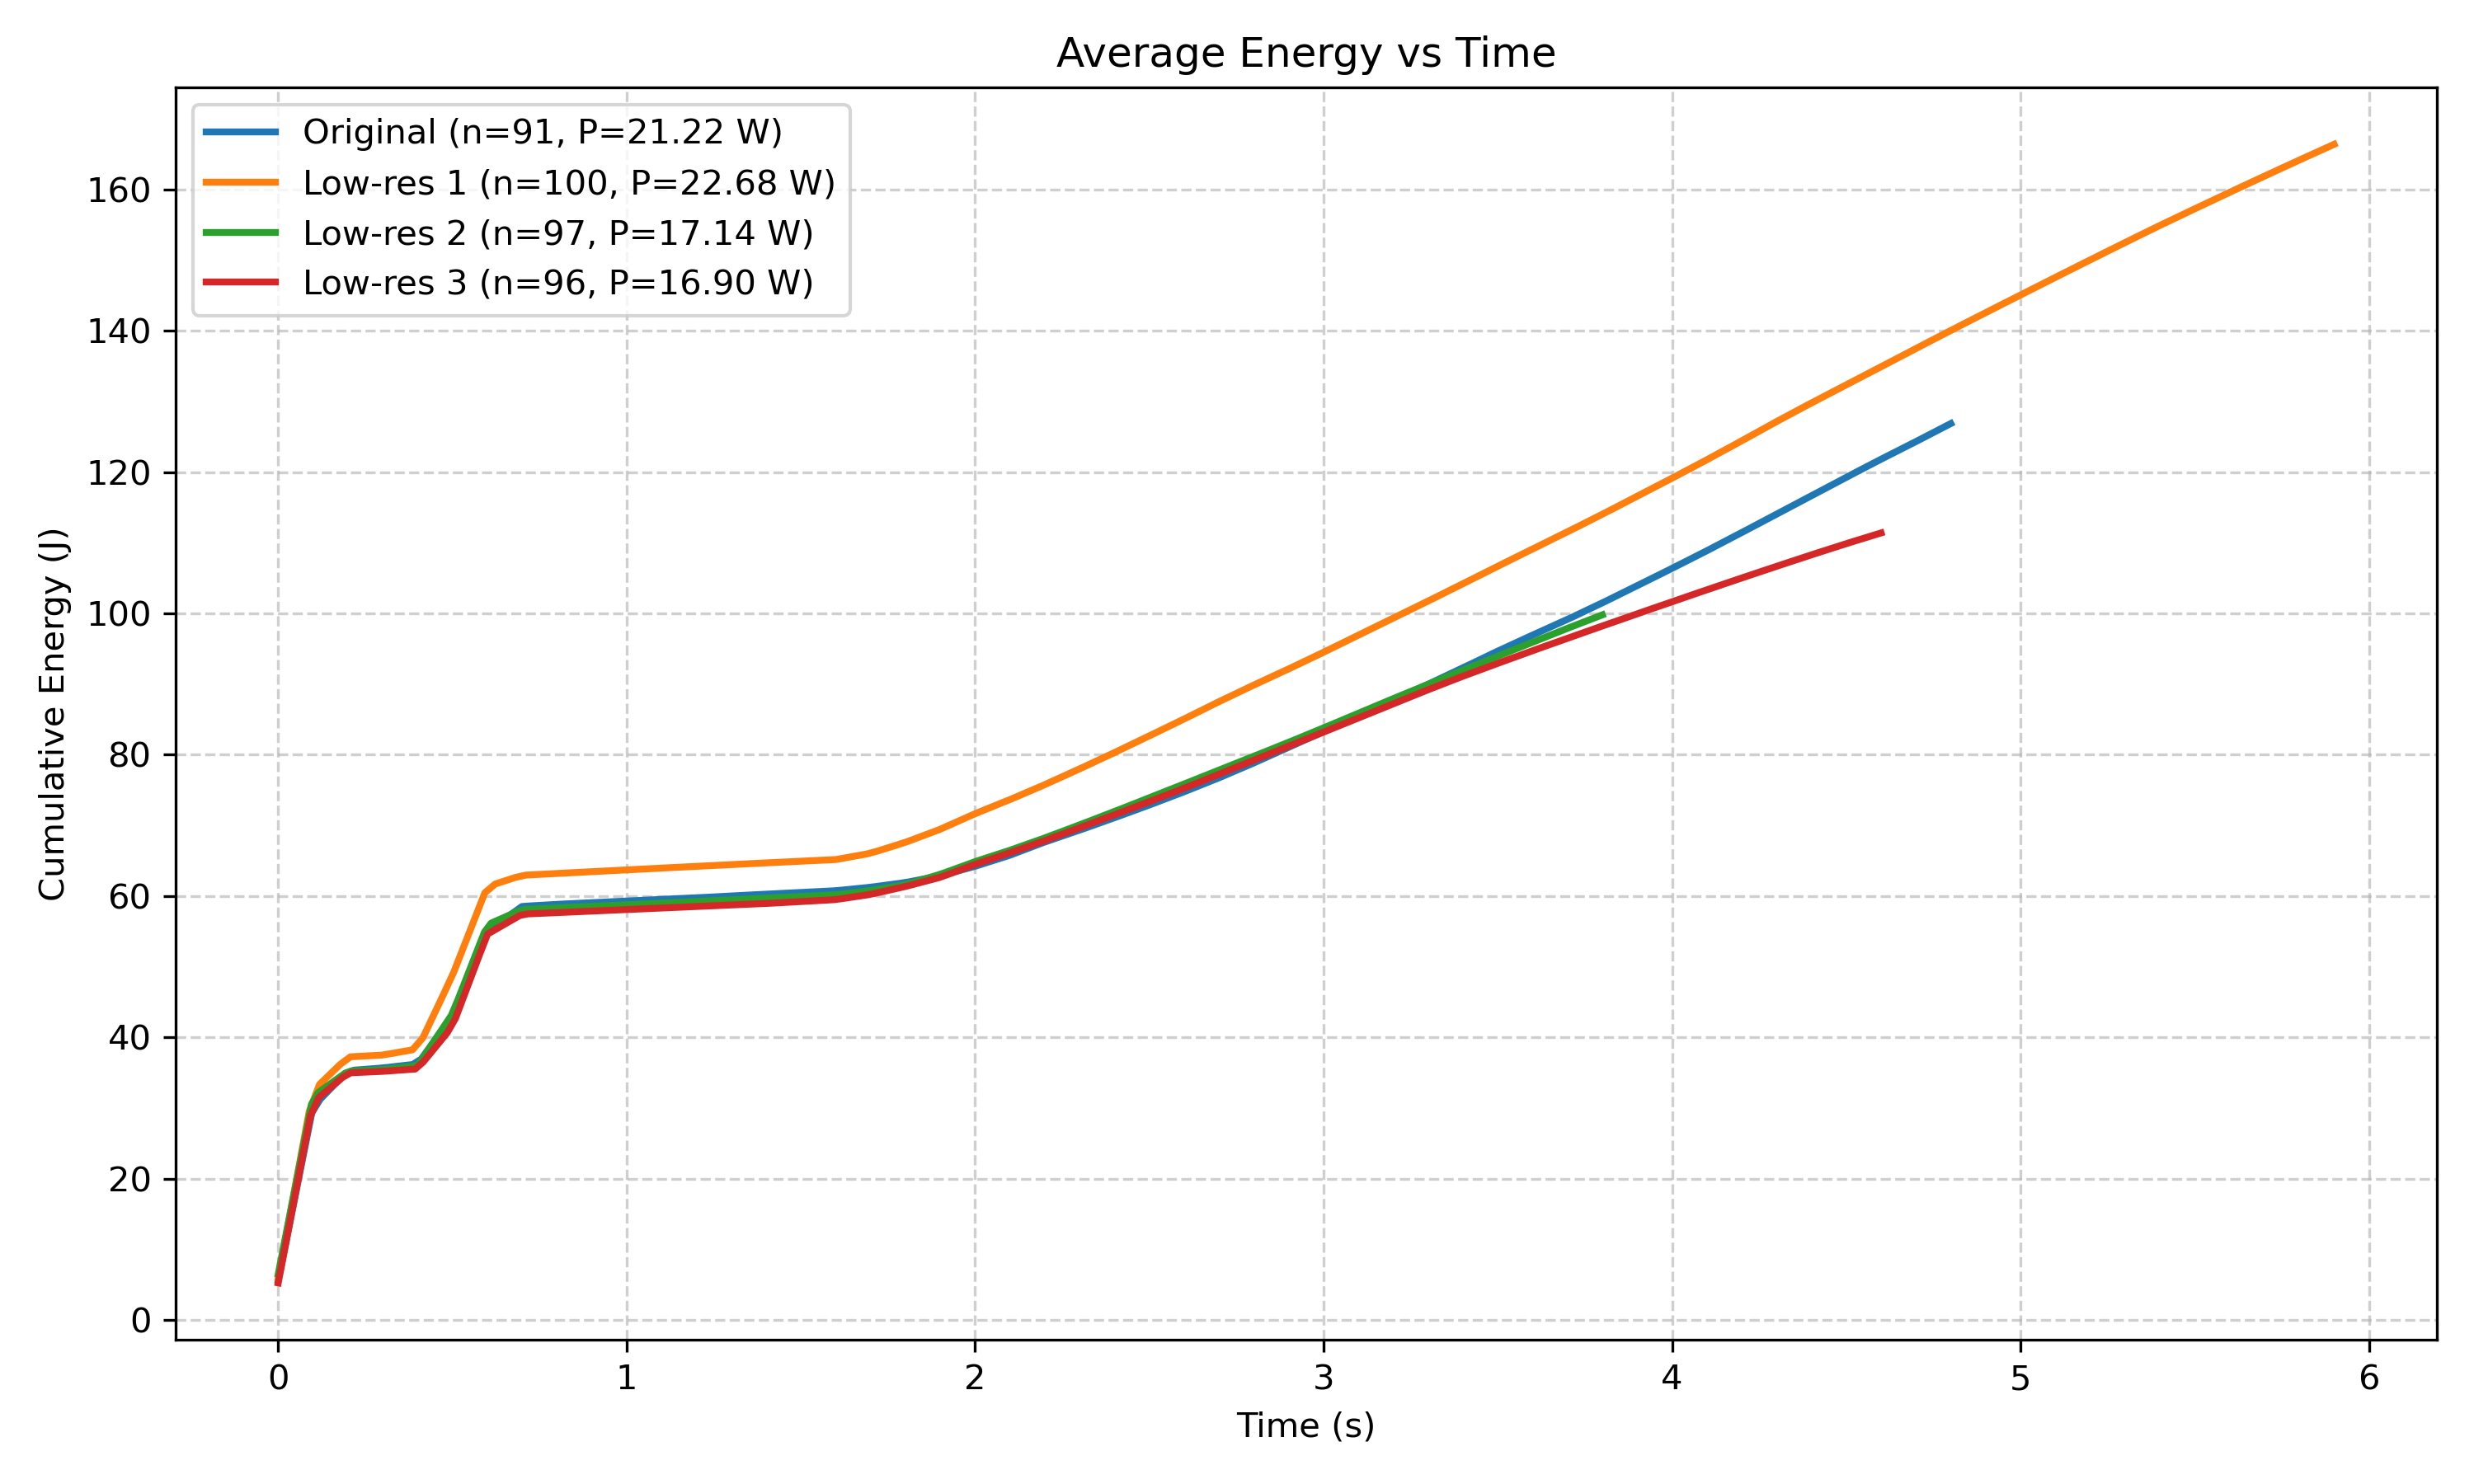
\includegraphics[width=1\textwidth]{images/results/time/power_signature.png}
    \caption{Average cumulative energy-time plot of ensembles with different resolutions.}
    \label{fig:power-signature}
\end{figure}

This behavior suggests that altering the spatial resolution of a hydrodynamic simulation does not simply decrease or increase the execution duration. Instead, it can actively alter the intensity of the hardware's power footprint. Because varying the computational workload appears to shift the baseline power rate, execution time alone may not reliably predict energy consumption across varying grid scales.

%%%%%%%%%%%%%%%%%%%%%%%%%%%%%%%%%%%%%%%%%%%%%%%%%%%%%%%%%%%%%%%%%%%%%%%%%

\section{Study 2: Physical Hazard Uncertainty Quantification}
\label{sec:res-study2}

To establish a baseline understanding of how topographic errors affect simulation accuracy, this study investigates the necessity of UQ within our flood case. The primary objective is to quantify how physical input noise propagates through the SynxFlow solver to alter the resulting spatial flood predictions.

\subsection{Experimental Setup}
Five separate Monte Carlo ensembles were generated, each applying a different level of spatially stationary Gaussian noise to the baseline Digital Elevation Model (DEM). The selected noise standard deviations, $\sigma \in \{0.05, 0.1, 0.2, 0.5, 1.0\}\,\text{m}$, were chosen to represent the real-world accuracy spectrum of various remote sensing technologies:
\begin{itemize}
    \item \textbf{0.05\,m}: Represents optimal drone mapping under ideal conditions, which can achieve absolute uncertainties as low as $\pm 0.05\,\text{m}$ \cite{VanderSluijs2026}.
    \item \textbf{0.1\,m}: Represents the industry standard for high-quality, drone-derived terrain maps. This value aligns with official accuracy standards for high-resolution geospatial data, even in lightly vegetated areas \cite{VanderSluijs2026, ASPRS2015Standards}.
    \item \textbf{0.2\,m}: Reflects the loss of accuracy that occurs in taller, dense vegetation, where the true ground is partially obscured from the sensor \cite{VanderSluijs2026}.
    \item \textbf{0.5\,m}: Represents severe elevation bias, such as when thick shrubs completely block the ground and are mistakenly recorded as solid terrain by the sensor \cite{VanderSluijs2026}.
    \item \textbf{1.0\,m}: Represents older or lower-resolution legacy datasets (such as aerial radar mapping), which typically exhibit vertical errors of $1.0$ to $2.0\,\text{meters}$ \cite{ASPRS2015Standards}.
\end{itemize}

Each of the five ensembles consists of $100$ equiprobable realizations. This sample size strikes a practical balance between statistical accuracy and computational cost. It provides enough data points for the statistical metrics to stabilize, while keeping the total execution time and energy requirements manageable for GPU-accelerated solvers.

To measure the physical impact of the input noise, the Quantity of Interest (QoI) was defined as the maximum water depth recorded at a specific spatial coordinate \texttt{[925.0, 605.0]}. 

This specific coordinate was selected because it represents a transitional flood zone. Coordinates situated in the center of a deep riverbed will inevitably flood across all iterations, exhibiting low variance, while coordinates on elevated topography will constantly remain dry. In contrast, a point located on the exact margin of the flood extent is highly sensitive to localized topographical noise. This approach mimics real-world challenges, such as evaluating the localized flood risk for a residential structure built on the absolute edge of a floodplain.

\subsection{Statistical Framework}
To quantify the degradation of physical predictions as input data quality drops, three statistical metrics were calculated for the water depth at the QoI across each ensemble:
\begin{itemize}
    \item \textbf{Mean ($\mu$):} Establishes the expected physical water depth (in meters) at the boundary coordinate for each noise tier.
    \item \textbf{Standard Deviation ($\sigma$):} Quantifies the absolute physical error introduced into the flow dynamics by the sensor noise.
    \item \textbf{Coefficient of Variation (CV):} Normalizes the physical error relative to the mean depth. High $\text{CV}$ percentages at larger noise levels (e.g., $\sigma \ge 0.5\,\text{m}$) suggest a decline in the simulation's predictive reliability.
\end{itemize}


\subsection{Results of Study 2}

Table \ref{tab:study2-results} summarizes the statistical impact of topographical uncertainty on the simulated water depth at the selected location. Within the context of this specific case study, the data reveals three key observations regarding how input errors propagate through the hydrodynamic solver.

\begin{table}[H]
  \centering
  \begin{tabular}{cccc}
    \toprule
    \textbf{$\sigma_{input}$ (m)} & \textbf{Mean (m)} & \textbf{Std. Dev (m)} & \textbf{CV (\%)} \\
    \midrule
    0.05 & 0.739 & $\pm 0.050$ & 6.78\% \\
    0.1  & 0.756 & $\pm 0.110$ & 14.50\% \\
    0.2  & 0.774 & $\pm 0.206$ & 26.61\% \\
    0.5  & 0.880 & $\pm 0.446$ & 50.71\% \\
    1.0  & 1.101 & $\pm 0.817$ & 74.21\% \\
    \bottomrule
  \end{tabular}
  \caption{Impact of input uncertainty $\sigma_{input}$ on the resulting water depth measurements.}
  \label{tab:study2-results}
\end{table}

As expected, increasing the topographical noise ($\sigma_{\text{input}}$) directly degrades the certainty of the physical simulation. At high quality sensor resolutions ($\sigma = 0.05\,\text{m}$ and $0.1\,\text{m}$), the model output remains relatively stable, showing a CV below 15\%. However, as the DEM accuracy drops to levels typical of dense vegetation or older legacy datasets ($\sigma \ge 0.5\,\text{m}$), the predictive confidence drops considerably. At $\sigma = 1.0\,\text{m}$, the standard deviation of the water depth reaches $\pm 0.817\,\text{m}$, resulting in a CV of 74.21\%. For this specific coordinate, a variance this large suggests that localized flood predictions may become unreliable for risk assessment, as the margin of error approaches the predicted flood depth itself.

While the increase of the standard deviation was anticipated, the behavior of the expected water depth provides an interesting observation. Because the injected Gaussian noise was strictly zero-mean ($\mu = 0$), one might expect the resulting mean water depth to remain relatively constant across the ensembles, with only the variance increasing. Instead, the data points to a potential systematic positive bias. The mean water depth rises from $0.739\,\text{m}$ at the lowest noise tier to $1.101\,\text{m}$ at the highest.

This implies that, in this specific simulation, topographical noise causes more than just random fluctuations. The bumps and dips introduced by the noise likely act as synthetic dams and sinks and these artificial obstructions prevent natural drainage. As a result, the water pools and backs up into the gauge location, leading to the higher localized flood depths observed here.

These initial results highlight why deterministic, single-run hazard assessments can potentially be misleading, especially in locations near riverbeds. Therefore, executing UQ serves as a valuable tool for understanding the true reliability of a flood map.



%%%%%%%%%%%%%%%%%%%%%%%%%%%%%%%%%%%%%%%%%%%%%%%%%%%%%%%%%%%%%%%%%%%%%%%%%

\section{Study 3: Energy Consumption Uncertainty Propagation}
\label{sec:res-study3}

The final study assesses how physical input uncertainty propagates into computational energy variability. This study addresses Sub-question 3, by evaluating whether the topographic noise injected into the digital elevation model inherently alters the total process-attributed energy required to solve the hydrodynamic equations.

\subsection{Experimental Setup}
\label{sec:res-study3-setup}

To ensure a proper comparison, this study analyzes the exact same five Monte Carlo ensembles ($\sigma \in \{0.05, 0.1, 0.2, 0.5, 1.0\}\,\text{m}$) generated in \hyperref[sec:res-study2]{Study 2}.

Because the baseline simulation parameters remain identical across all runs, any observed change in energy consumption is mathematically isolated. This ensures that variations in power draw are caused by the GPU solver solving altered DEMs.

\subsection{Statistical Framework}
To quantify this variation, the resulting energy telemetry for each noise tier is evaluated using three specific statistical metrics:

\paragraph{Mean ($\mu$):}
As the standard deviation of the input noise ($\sigma$) increases, the simulated terrain becomes artificially "rougher," characterized by synthetic bumps and dips. To remain mathematically stable when water flows over steep or irregular gradients, hydrodynamic solvers like SynxFlow must rely on adaptive timestepping. Rougher terrain forces the solver to take smaller timesteps to solve the flow.

\paragraph{Standard Deviation ($\text{Std. Dev.}$):}
The standard deviation measures the spread of the energy in Joules. This metric quantifies how much the power draw swings from one individual iteration to the next, even when the overall noise distribution ($\sigma$) remains the same.

\paragraph{90\% Confidence Interval (5th and 95th Percentiles):}
To highlight the challenge this variance poses for large-scale risk assessment, the 90\% confidence interval of the total energy consumption is calculated. In shared HPC environments, researchers must allocate strict, predictable power and time budgets. If the upper bound (95th percentile) of the energy consumption diverges significantly from the mean at higher noise levels, it signals that running UQ ensembles can be unpredictable. This signals that one may not be able to simply profile a single iteration and accurately predict the maximum energy budget required for the full stochastic ensemble.

\subsection{Results of Study 3}

The initial evaluation of energy uncertainty (Run 1) analyzed a 100-iteration Monte Carlo ensemble for each noise tier. As shown in Figure~\ref{fig:energy-uq-boxplot} and summarized in Table~\ref{tab:run1-energy-stats}, the findings from this first execution window suggested that as topographic noise ($\sigma$) increased, both the average energy consumption and the run-to-run variance expanded. For example, the mean energy rose from $184.78\,\text{J}$ at $\sigma = 0.05\,\text{m}$ to $212.80\,\text{J}$ at $\sigma = 1.00\,\text{m}$, while the standard deviation nearly tripled from $\pm 19.71\,\text{J}$ to $\pm 55.75\,\text{J}$.

\begin{figure}[htbp]
  \centering
  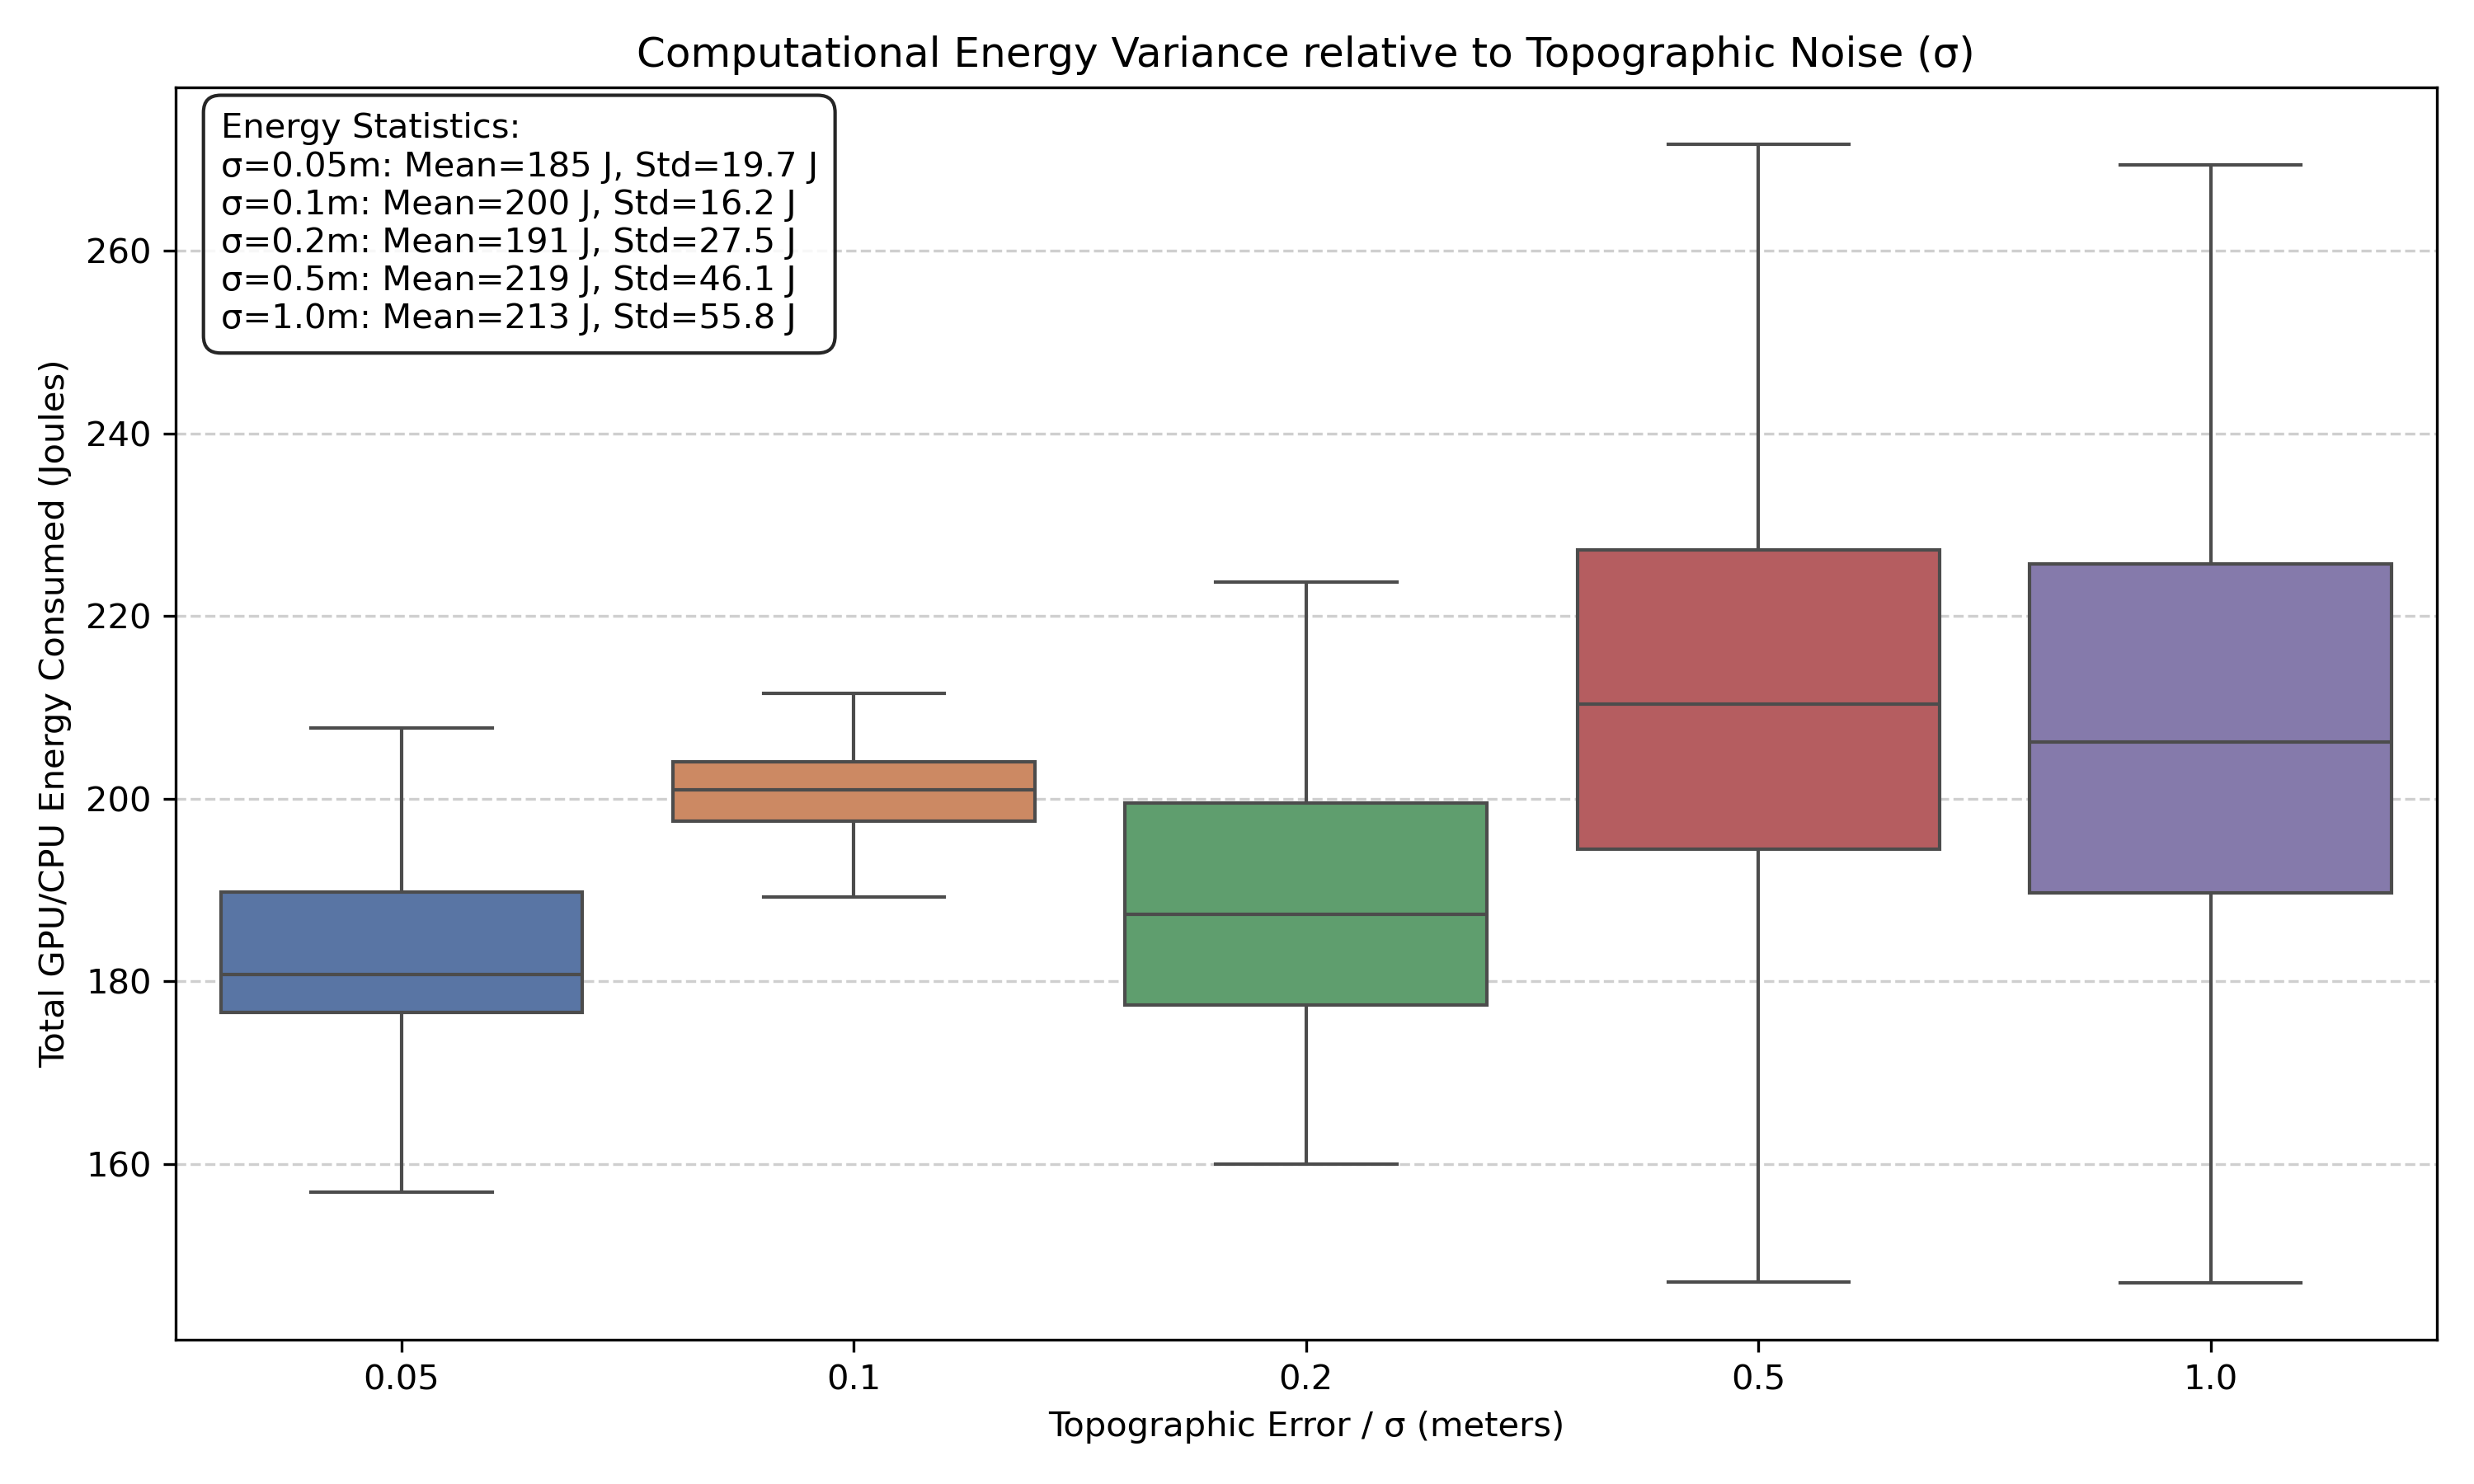
\includegraphics[width=1\textwidth]{images/results/uq/energy_uq_boxplot.png}
  \caption{Boxplots of total energy consumption for each topographic noise level for run 1}
  \label{fig:energy-uq-boxplot}
\end{figure}

\begin{table}[htbp]
\centering
\begin{tabular}{lcccc}
\toprule
\textbf{Topographic Noise ($\sigma$)} & \textbf{Mean ($\mu$)} & \textbf{Median} & \textbf{Std. Dev.} & \textbf{90\% Confidence Interval} \\
\midrule
$0.05\,\text{m}$ & $184.78\,\text{J}$ & $180.73\,\text{J}$ & $\pm 19.71\,\text{J}$ & $[169.25\,\text{J}, 207.33\,\text{J}]$ \\
$0.10\,\text{m}$ & $199.81\,\text{J}$ & $200.97\,\text{J}$ & $\pm 16.24\,\text{J}$ & $[176.86\,\text{J}, 211.62\,\text{J}]$ \\
$0.20\,\text{m}$ & $191.38\,\text{J}$ & $187.31\,\text{J}$ & $\pm 27.48\,\text{J}$ & $[167.91\,\text{J}, 220.32\,\text{J}]$ \\
$0.50\,\text{m}$ & $219.28\,\text{J}$ & $210.33\,\text{J}$ & $\pm 46.09\,\text{J}$ & $[152.31\,\text{J}, 319.68\,\text{J}]$ \\
$1.00\,\text{m}$ & $212.80\,\text{J}$ & $206.24\,\text{J}$ & $\pm 55.75\,\text{J}$ & $[147.81\,\text{J}, 293.47\,\text{J}]$ \\
\bottomrule
\end{tabular}
\caption{Statistical summary of total computational energy consumption for Run 1 (100 iterations).}
\label{tab:run1-energy-stats}
\end{table}

However, as demonstrated in \hyperref[sec:res-study1]{Study 1}, energy metrics in a shared HPC environment can be susceptible to background traffic. To verify whether the energy profile observed in Run 1 was an inherent property of the solver or just a reflection of the cluster's state during that specific execution window, the exact same experimental setup was duplicated in a separate, independent cluster allocation (Run 2).

\begin{figure}[htbp]
  \centering
  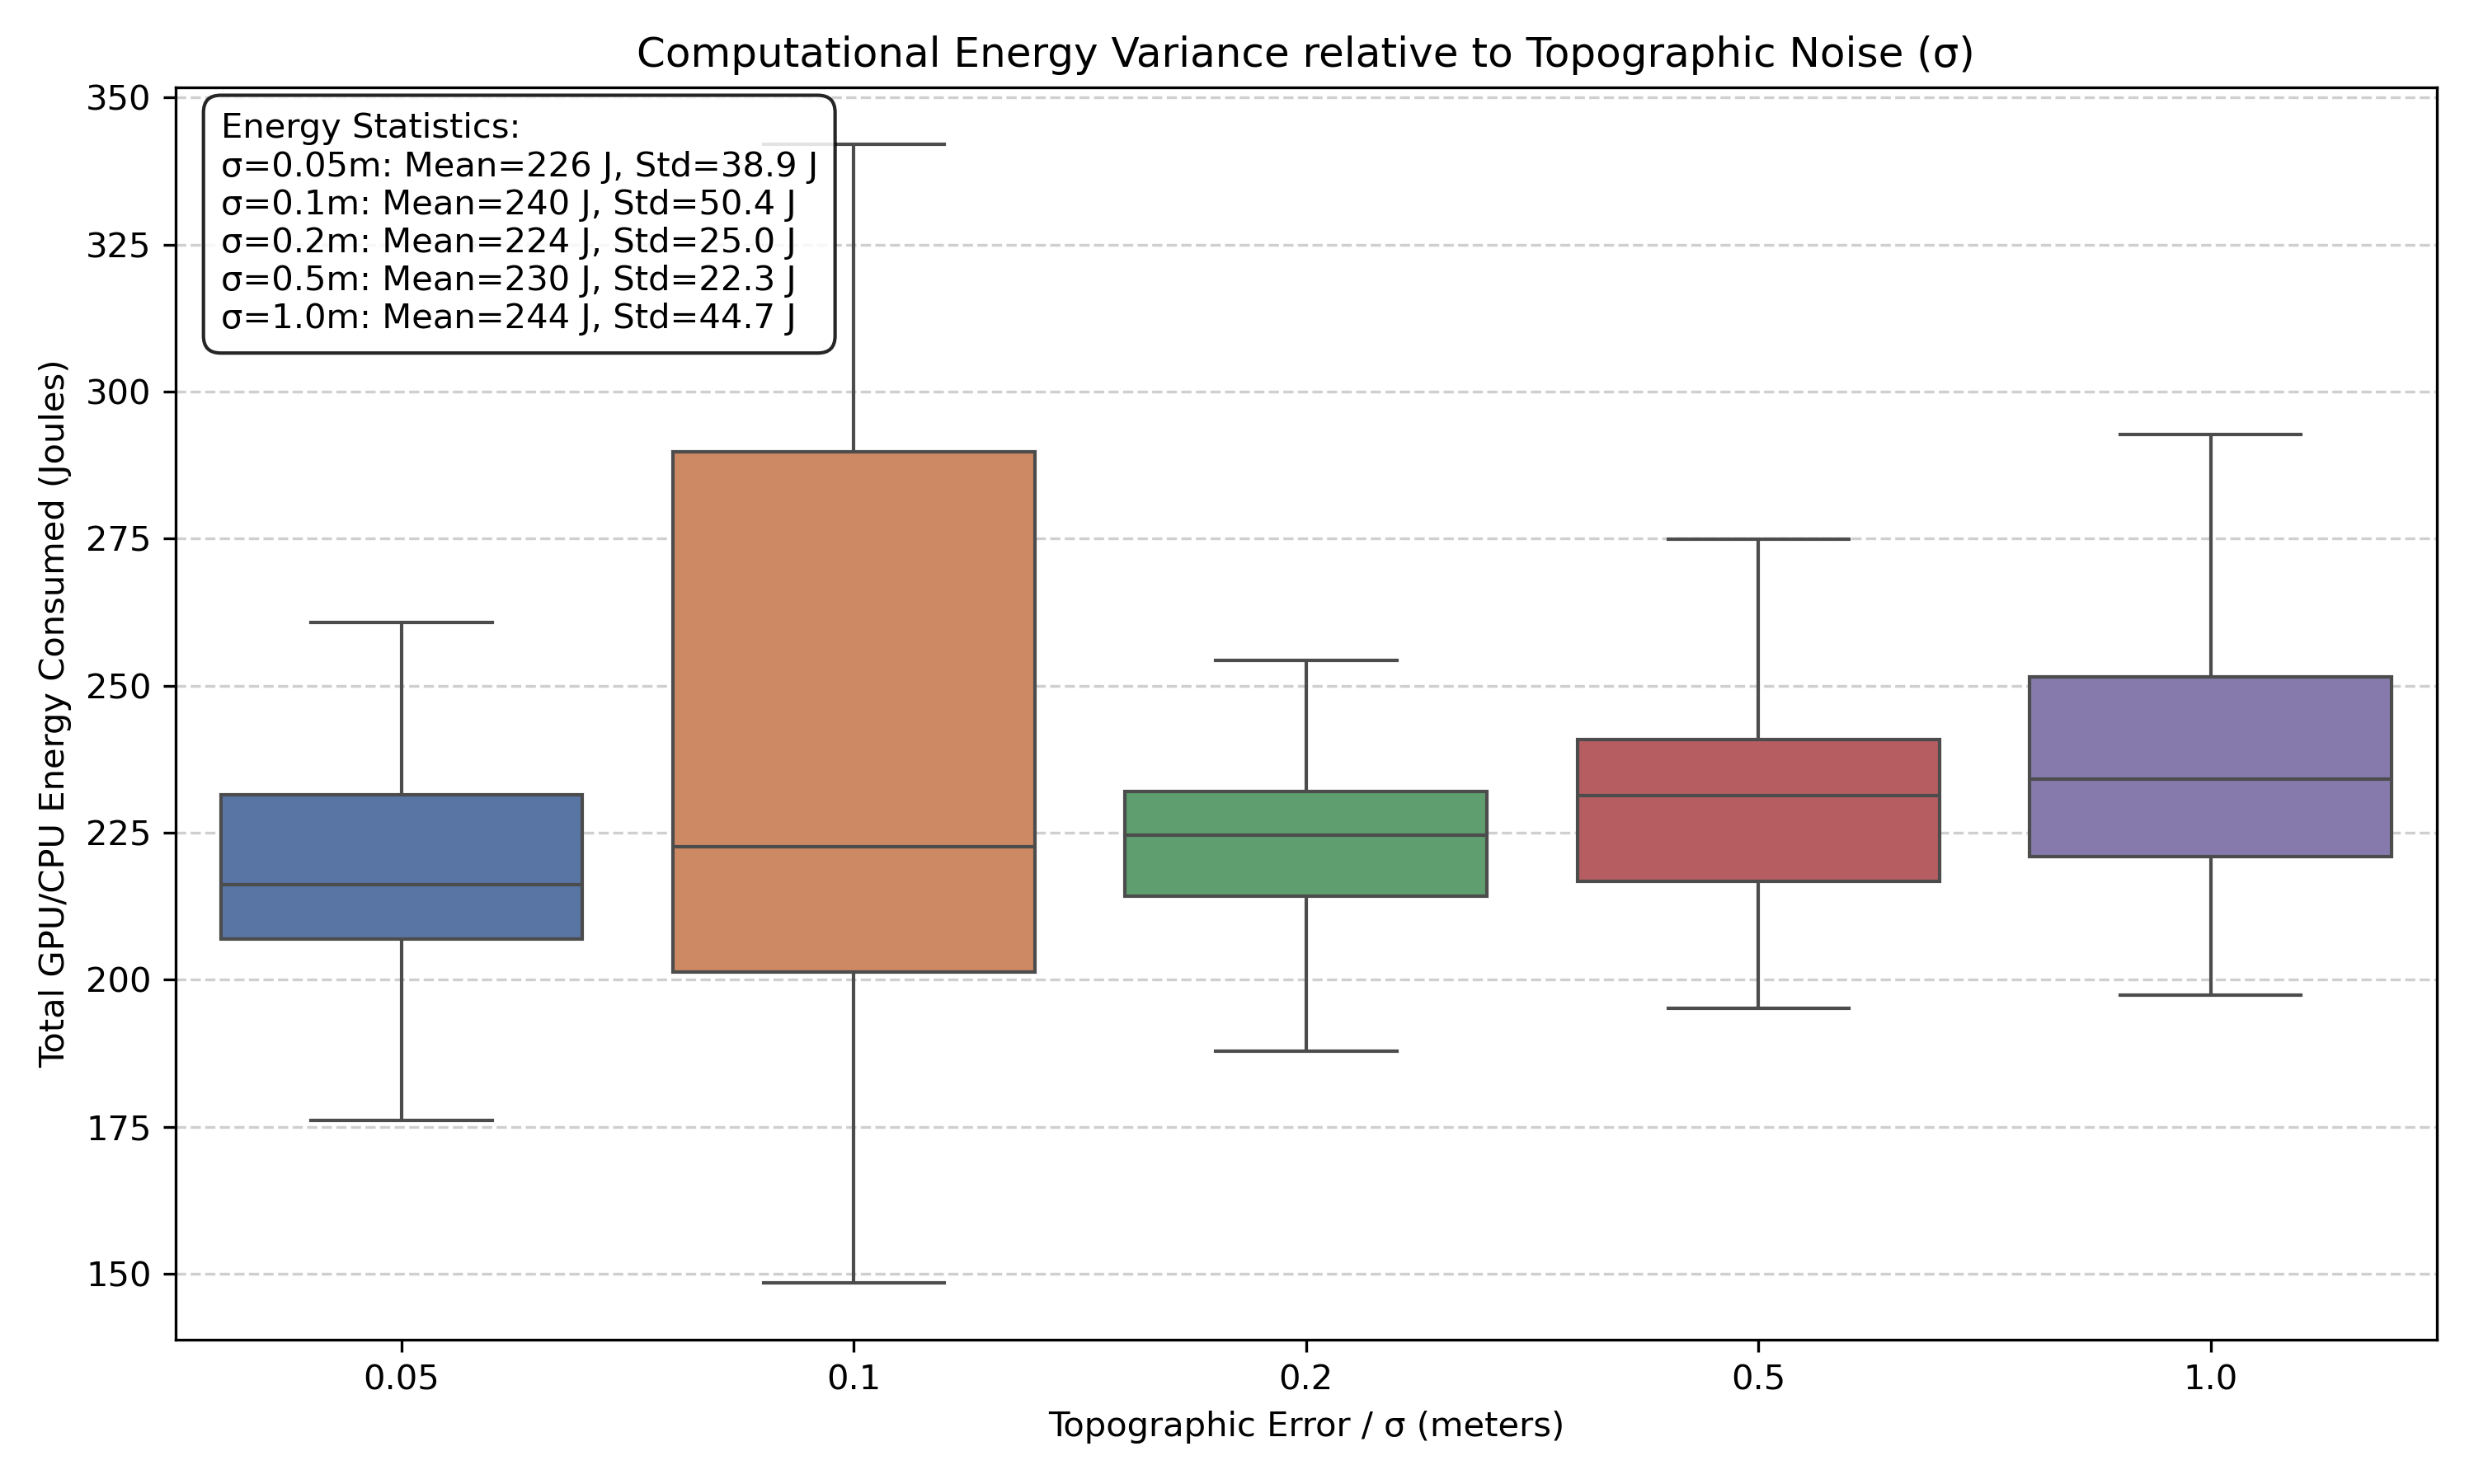
\includegraphics[width=1\textwidth]{images/results/uq/energy_uq_boxplot2.png}
  \caption{Boxplots of total energy consumption for each topographic noise level for run 2}
  \label{fig:energy-uq-boxplot2}
\end{figure}

\begin{table}[htbp]
\centering
\begin{tabular}{lcccc}
\toprule
\textbf{Topographic Noise ($\sigma$)} & \textbf{Mean ($\mu$)} & \textbf{Median} & \textbf{Std. Dev.} & \textbf{90\% Confidence Interval} \\
\midrule
$0.05\,\text{m}$ & $226.40\,\text{J}$ & $216.10\,\text{J}$ & $\pm 38.88\,\text{J}$ & $[183.00\,\text{J}, 319.78\,\text{J}]$ \\
$0.10\,\text{m}$ & $239.76\,\text{J}$ & $222.58\,\text{J}$ & $\pm 50.42\,\text{J}$ & $[182.70\,\text{J}, 332.58\,\text{J}]$ \\
$0.20\,\text{m}$ & $224.47\,\text{J}$ & $224.51\,\text{J}$ & $\pm 24.96\,\text{J}$ & $[189.88\,\text{J}, 255.58\,\text{J}]$ \\
$0.50\,\text{m}$ & $230.38\,\text{J}$ & $231.25\,\text{J}$ & $\pm 22.30\,\text{J}$ & $[202.45\,\text{J}, 259.73\,\text{J}]$ \\
$1.00\,\text{m}$ & $244.44\,\text{J}$ & $234.16\,\text{J}$ & $\pm 44.74\,\text{J}$ & $[210.16\,\text{J}, 331.28\,\text{J}]$ \\
\bottomrule
\end{tabular}
\caption{Statistical summary of total computational energy consumption for Run 2 (100 iterations).}
\label{tab:run2-energy-stats}
\end{table}


The telemetry from Run 2, detailed in Figure~\ref{fig:energy-uq-boxplot2} and Table~\ref{tab:run2-energy-stats}, also signals the impact of hardware volatility. While Run 2 exhibited similar internal trends regarding the expansion of variance, its overall baseline energy footprint was consistently higher across all tiers. For instance, at the $\sigma = 0.05\,\text{m}$ tier, the mean energy jumped from $184.78\,\text{J}$ in Run 1 to $226.40\,\text{J}$ in Run 2. Furthermore, Run 2 contains a striking anomaly at the $\sigma = 0.10\,\text{m}$ noise level. Despite representing a high-quality terrain input, this tier recorded a disproportionately high mean of $240\,\text{J}$ and the largest standard deviation of the run at $\pm 50.4\,\text{J}$. Because \hyperref[sec:res-study1]{Study 1} established that idle cluster stalls reduce dynamic power rates rather than surging computational energy, this elevated energy footprint is unlikely to stem from pure hardware idling. Instead, it suggests that specific DEMs within this tier may have triggered aggressive adaptive timestepping in the solver. These discrepancies illustrate that baseline energy profiles can fluctuate significantly between execution windows due to a combination of input-uncertainty and cluster conditions.

Because evaluating a single execution window might lead to biased conclusions regarding total operational cost, the telemetry from both runs was merged into a single 200-iteration ensemble per noise tier. This combined dataset aims to mitigate cluster-induced variance and establish a more generalized understanding of the solver's energy behavior. Figure~\ref{fig:energy-uq-boxplot-combined} and Table~\ref{tab:combined-energy-stats} summarize the statistical findings for this merged dataset.


\begin{figure}[htbp]
  \centering
  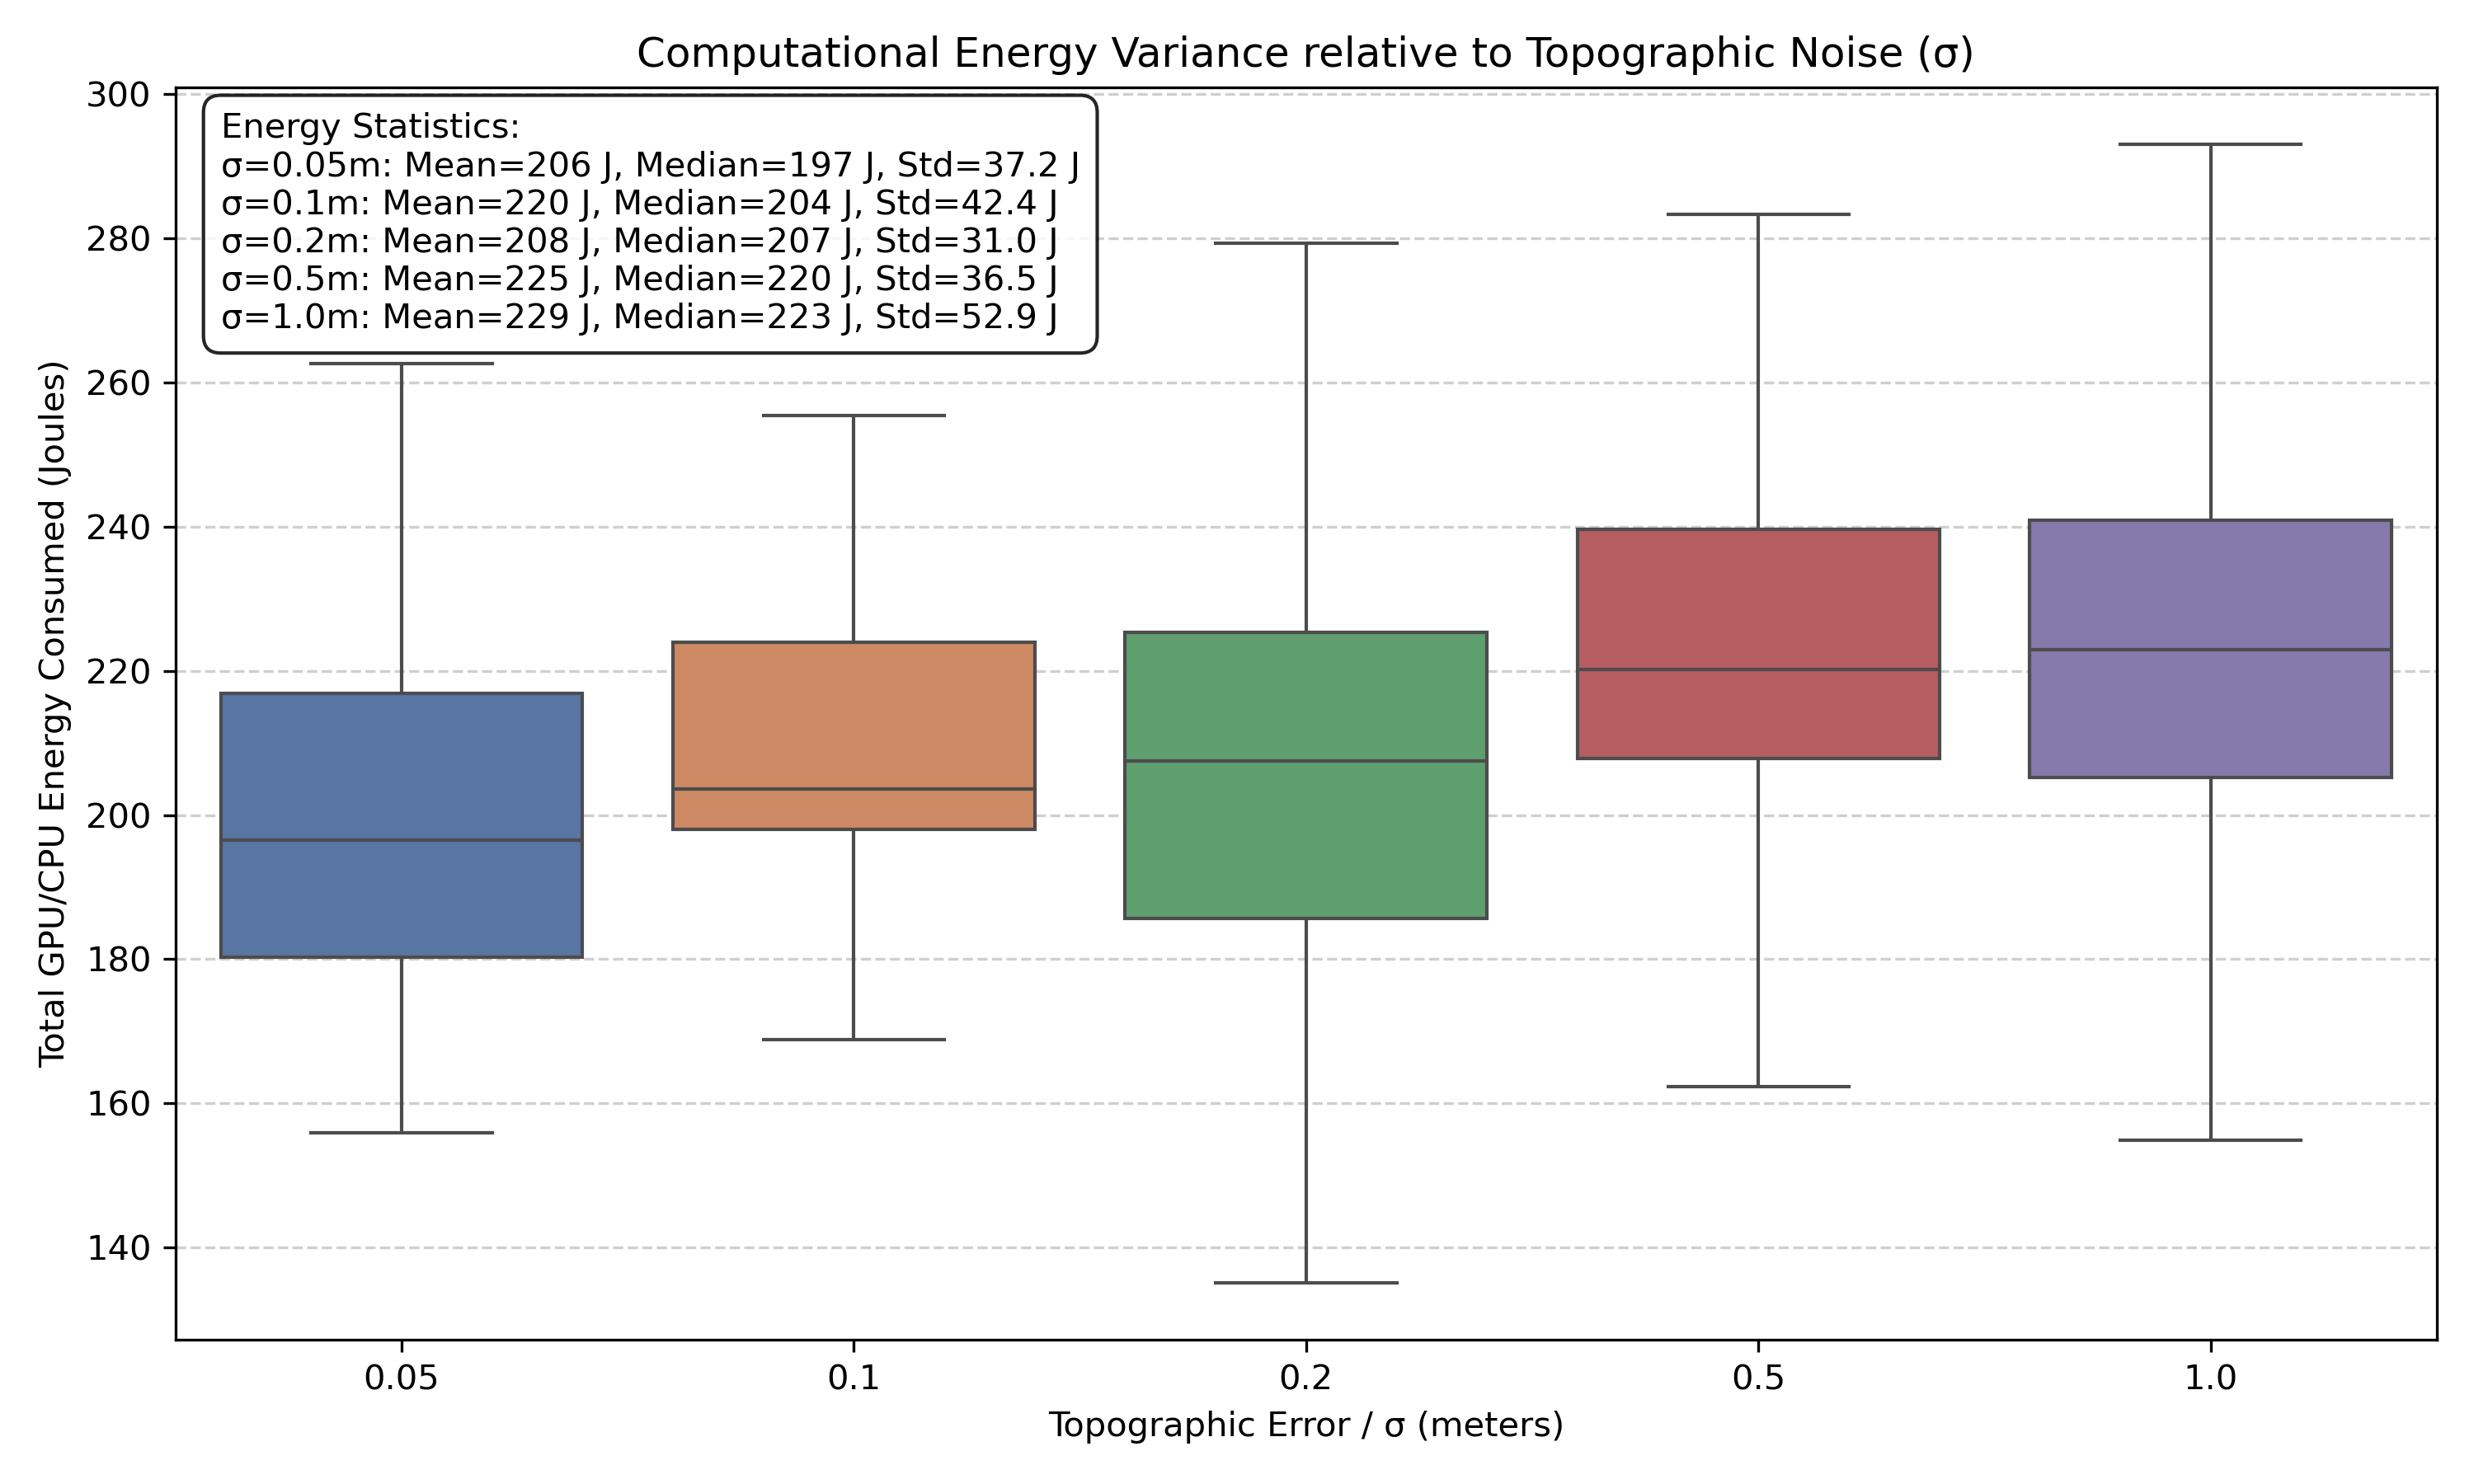
\includegraphics[width=1\textwidth]{images/results/uq/energy_uq_boxplot_combined.png}
  \caption{Boxplots of total energy consumption for combined results of runs 1 and 2}
  \label{fig:energy-uq-boxplot-combined}
\end{figure}

\begin{table}[htbp]
\centering
\begin{tabular}{lcccc}
\toprule
\textbf{Topographic Noise ($\sigma$)} & \textbf{Mean ($\mu$)} & \textbf{Median} & \textbf{Std. Dev.} & \textbf{90\% Confidence Interval} \\
\midrule
$0.05\,\text{m}$ & $205.59\,\text{J}$ & $196.53\,\text{J}$ & $\pm 37.15\,\text{J}$ & $[171.09\,\text{J}, 301.03\,\text{J}]$ \\
$0.10\,\text{m}$ & $219.79\,\text{J}$ & $203.66\,\text{J}$ & $\pm 42.39\,\text{J}$ & $[181.82\,\text{J}, 318.61\,\text{J}]$ \\
$0.20\,\text{m}$ & $207.92\,\text{J}$ & $207.50\,\text{J}$ & $\pm 31.00\,\text{J}$ & $[172.34\,\text{J}, 249.60\,\text{J}]$ \\
$0.50\,\text{m}$ & $224.83\,\text{J}$ & $220.15\,\text{J}$ & $\pm 36.54\,\text{J}$ & $[170.81\,\text{J}, 299.63\,\text{J}]$ \\
$1.00\,\text{m}$ & $228.62\,\text{J}$ & $222.91\,\text{J}$ & $\pm 52.85\,\text{J}$ & $[167.94\,\text{J}, 312.16\,\text{J}]$ \\
\bottomrule
\end{tabular}
\caption{Statistical summary of total computational energy consumption for the combined 200-iteration ensembles.}
\label{tab:combined-energy-stats}
\end{table}

The combined telemetry data offers three key observations regarding how topographic uncertainty might propagate into computational energy metrics within the scope of this specific study.

By evaluating both the median and the mean, the data reveals a distinction between the solver's theoretical efficiency and its actual operational cost. Across the ensembles, the mean is generally higher than the median. This right-skewed distribution suggests that while the solver's baseline energy cost remains relatively stable under typical conditions (represented by the median), a combination of transient cluster delays and complex local flow iterations creates a long tail of higher-energy outliers that elevate the mean energy consumption. Additionally, both metrics show a general upward trend as topographic noise increases. This suggests that as the injected noise creates artificially steep gradients, and SynxFlow likely shrinks its adaptive timestep to maintain numerical stability, which appears to incrementally increase the overall energy required to solve the simulation.

Beyond altering the average energy cost, higher topographic noise appears to degrade the predictability of the solver's energy footprint. The spread of energy consumption generally increases as the input noise increases. For the $0.05\,\text{m}$ and $0.20\,\text{m}$ tiers, the standard deviations are $37.15\,\text{J}$ and $31.00\,\text{J}$, respectively. However, at the $1.00\,\text{m}$ noise tier, the standard deviation expands to $52.85\,\text{J}$. This indicates that when a digital elevation model is highly uncertain, the computational energy required to process it might also become highly uncertain, leading to more run-to-run variance even within the exact same noise distribution.

The expansion of the 90\% confidence interval highlights a potential challenge for energy estimation in HPC environments. The combined data shows that at the $1.00\,\text{m}$ noise tier, the 95th percentile upper bound reaches $312.16\,\text{J}$, which is nearly $84\,\text{J}$ higher than the mean. Within the context of this study, this suggests that relying on a single deterministic profile to predict the maximum energy budget for a full stochastic ensemble might result in under-allocation. Consequently, safety margins for computational budgets may need to be scaled dynamically based on the quality of the input data, with poorer input data potentially requiring a wider safety net.

  \chapter{Summary and Future Work}\label{ch:summary}

This report addressed the gap between geohazard uncertainty quantification and computational energy profiling. By coupling the SynxFlow hydrodynamic solver with the Alumet telemetry framework, this work transitioned from relying on execution time as a proxy to directly measuring process-isolated energy consumption for stochastic flood simulations. This chapter summarizes the key findings, acknowledges experimental limitations, and outlines future research directions.

%%%%%%%%%%%%%%%%%%%%%%%%%%%%%%%%%%%%%%%%%%%%%%%%%%%%%%%%%%%%%%%%%%%%%%%%
\section{Summary}\label{sec:summary}

This research investigated how input data uncertainty and execution environment volatility impact the energy predictability of GPU-accelerated flood solvers. The core research questions from Section~\ref{sec:research-questions} were addressed as follows:
  
\begin{itemize}
    \item[\textit{RQ1}] \textbf{Methodologies for process-level energy attribution:} A custom Python framework was developed to integrate SynxFlow with Alumet. By utilizing dynamic Process ID tracking and scaling hardware power by utilization percentages, this methodology isolated the solver's true energy footprint from shared cluster noise.
    
    \item[\textit{RQ2}] \textbf{Execution time as an energy proxy:} Preliminary results indicated that execution time may be an unreliable standalone proxy for computational energy in this context. Welch's t-tests suggested that altering the computational grid's spatial resolution can shift the hardware's dynamic power intensity. Time-to-solution might not fully capture this energy variability, as power rates appeared to fluctuate based on grid-to-GPU alignment.

    \item[\textit{RQ3}] \textbf{Uncertainty propagation to energy variability:} Initial observations suggested that as spatial input uncertainty ($\sigma$) increases, both the average computational energy and run-to-run variance show a tendency to expand. Rougher terrain may trigger adaptive timestepping, potentially producing right-skewed energy distributions. This indicates that highly uncertain DEMs could lead to highly uncertain energy footprints, suggesting that single deterministic profiles might underestimate the energy requirements of stochastic ensembles.
\end{itemize}
%%%%%%%%%%%%%%%%%%%%%%%%%%%%%%%%%%%%%%%%%%%%%%%%%%%%%%%%%%%%%%%%%%%%%%%%

\section{Limitations}
\label{sec:limitations}

While establishing a foundational link between input uncertainty and energy consumption, this study has several boundaries. First, the simplified error modeling relies on a zero-mean Gaussian noise model ($\epsilon \sim \mathcal{N}(0, \sigma^2)$), which assumes isotropic errors and oversimplifies the spatially correlated and biased errors of real-world remote sensing. Second, the scope of the scenario is limited, as the findings stem from a single flood simulation. Consequently, the observed non-linear hydrodynamic effects may not uniformly apply to varying catchments or urban floodplains.

Additionally, due to computational expense, the ensemble sizes were restricted to 100 iterations. While this sample size captures primary trends, it may be insufficient to fully stabilize extreme tail behaviors within the energy distributions. Finally, the observed power shifts are inherently tied to the hardware specificity of the Gaia compute cluster and its NVIDIA GPUs, meaning these exact energy dynamics may vary across different computing architectures.

%%%%%%%%%%%%%%%%%%%%%%%%%%%%%%%%%%%%%%%%%%%%%%%%%%%%%%%%%%%%%%%%%%%%%%%%
\section{Future Work}
\label{sec:future-work}

The findings of this thesis open several promising directions for further research. First, future studies must improve the error model by incorporating spatially correlated noise alongside a negative bias shift. Because spaceborne sensors frequently overestimate ground heights by capturing vegetation and buildings instead of bare earth \cite{Meadows2024}, an accurate error model must simulate the removal of this positive sensor bias by lowering the elevation values in obstructed areas.

Furthermore, the topographic scope of the framework should be expanded. Testing the methodology on diverse flood cases and different DEMs will help determine if specific terrain features inherently demand higher adaptive energy costs. Finally, scaling the Monte Carlo simulations to larger ensembles is necessary to observe if the variability in energy consumption fully stabilizes. Capturing this stabilization is critical for establishing reliable, carbon-aware HPC scheduling limits.

\appendix
  \include{sources/appendix}

% This ensures that the subsequent sections are being included as root
% items in the bookmark structure of your PDF reader.
\bookmarksetup{startatroot}
\backmatter
  \printbibliography

\end{document}
